\documentclass[12pt,a4paper,twoside]{report}

% ==================================================
% Encodage et langue
% ==================================================

\usepackage[utf8]{inputenc}
\usepackage[T1]{fontenc}
\usepackage[french]{babel}

% ==================================================
% Police et géométrie
% ==================================================

\usepackage{lmodern}
\usepackage{setspace}
\usepackage{listings}
\usepackage{xcolor}

\usepackage[
    top=2.5cm,
    bottom=2.5cm,
    left=2.5cm,
    right=2.5cm
]{geometry}

% ==================================================
% Graphiques et figures
% ==================================================

\usepackage{microtype}
\usepackage{graphicx}
\usepackage{float}
\usepackage{caption}
\usepackage{subcaption}
\usepackage{pdflscape}
\usepackage{pdfpages}

% ==================================================
% Tableaux
% ==================================================

\usepackage{tabularx}
\usepackage{makecell}
\usepackage{array}
\usepackage{ragged2e}
\usepackage{longtable}
\usepackage{multirow}
\usepackage[table]{xcolor}
\usepackage{colortbl}
\usepackage{booktabs}

% ==================================================
% Mathématiques
% ==================================================

\usepackage{amsmath}
\usepackage{amssymb}

% ==================================================
% Mise en page et styles
% ==================================================

\usepackage{titlesec}
\usepackage{xcolor}
\usepackage{enumitem}
\usepackage{indentfirst}
\usepackage{pifont}
\usepackage{varioref}
\usepackage[hyphens]{url}

% ==================================================
% Hyperliens
% ==================================================

\usepackage[
    colorlinks=true,
    linkcolor=black,
    citecolor=black,
    urlcolor=blue
]{hyperref}

% ==================================================
% Gestion des headers/footers
% ==================================================

\usepackage{fancyhdr}

\setlength{\headheight}{15pt}

% Réduction des problèmes Overfull/Underfull
\emergencystretch=3em
\hfuzz=5pt
\vbadness=10000
\hbadness=10000

% ==================================================
% Numérotation figures/tableaux
% ==================================================

\usepackage{chngcntr}

\counterwithout{figure}{chapter}
\counterwithout{table}{chapter}
\counterwithin{section}{chapter}

% ==================================================
% Espacements
% ==================================================

\renewcommand{\arraystretch}{1.3}

\setlength{\floatsep}{5pt plus 2pt minus 2pt}
\setlength{\textfloatsep}{5pt plus 2pt minus 2pt}
\setlength{\intextsep}{5pt plus 2pt minus 2pt}

% ==================================================
% Style headers/footers
% ==================================================

\fancypagestyle{plain}{
    \fancyhf{}
    \fancyfoot[C]{\thepage}
    \renewcommand{\headrulewidth}{0pt}
    \renewcommand{\footrulewidth}{0pt}
}

\pagestyle{fancy}

\fancyhf{}

\fancyhead[LE]{\nouppercase{\leftmark}}
\fancyhead[RO]{\nouppercase{\rightmark}}

\fancyfoot[C]{\thepage}

\renewcommand{\headrulewidth}{0.5pt}

% ==================================================
% Style des titres
% ==================================================

\titleformat{\chapter}[display]
{\normalfont\Huge\bfseries\centering}
{\chaptername\ \thechapter}
{20pt}
{\Huge}

\titlespacing*{\chapter}
{0pt}
{0pt}
{20pt}

% ----------------------------

\titleformat{\section}
{\normalfont\Large\bfseries}
{\thesection}
{1em}
{}

% ----------------------------

\titleformat{\subsection}
{\normalfont\large\bfseries}
{\thesubsection}
{1em}
{}

% ----------------------------

\titleformat{\subsubsection}
{\normalfont\normalsize\bfseries}
{\thesubsubsection}
{1em}
{}

% ==================================================
% Numérotation sections
% ==================================================

\renewcommand{\thesection}{\thechapter.\arabic{section}}
\renewcommand{\thesubsection}{\thesection.\arabic{subsection}}
\renewcommand{\thesubsubsection}{\thesubsection.\arabic{subsubsection}}

% Suppress blank pages inserted by \cleardoublepage (twoside mode)
\let\cleardoublepage\clearpage

% Prevent LaTeX from stretching content vertically to fill pages (avoids large gaps)
\raggedbottom

% ==================================================
% Début document
% ==================================================

\begin{document}

% ==================================================
% Page de garde
% ==================================================

\pagestyle{empty}

\begin{titlepage}
\begin{center}

\vspace*{0.5cm}

{\large \textbf{République Tunisienne}}\\[0.3em]
{\large \textbf{Ministère de l'Enseignement Supérieur et de la Recherche Scientifique}}\\[0.8em]

\textbf{Université de Monastir}\\[0.2em]
\textbf{Faculté des Sciences de Monastir}\\[1.5em]

\rule{\linewidth}{0.5pt}\\[1em]

{\Large \textbf{Projet de Fin d'Études}}\\[0.5em]
{\normalsize Pour l'obtention du diplôme de Licence / Master en Informatique}\\[1.2em]

\rule{\linewidth}{0.5pt}\\[1.2em]

{\LARGE \textbf{LexAI}}\\[0.5em]
{\large \textbf{Plateforme IA d'Analyse Automatisée}}\\[0.3em]
{\large \textbf{de la Conformité des Contrats Juridiques}}\\[1.8em]

% e-Tafakna logo
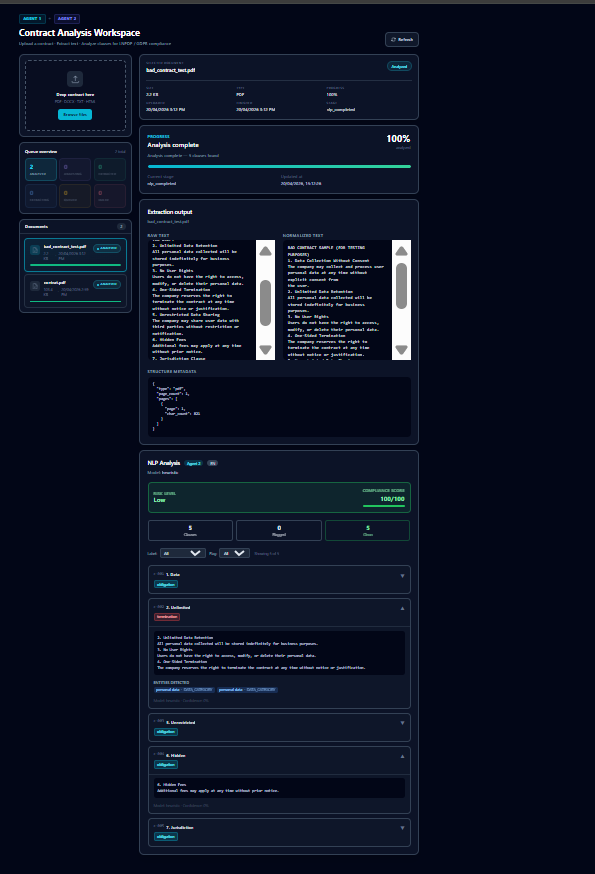
\includegraphics[width=5cm]{images/etafakna-logo}\\[1.5em]

\begin{tabular}{ll}
\textbf{Réalisé par :} & \textbf{Ala Missaoui} \\[0.5em]
\textbf{Entreprise d'accueil :} & \textbf{e-Tafakna} \\[0.5em]
\textbf{Encadrant académique :} & \textbf{Badreddine Guizani} \\[0.5em]
\textbf{Encadrante professionnelle :} & \textbf{Dhekra Ben Mahmoud} \\
\end{tabular}

\vfill

{\normalsize Année Universitaire 2025 -- 2026}

\end{center}
\end{titlepage}

% ==================================================
% Pages préliminaires
% ==================================================

% ==================================================
% Table des matières
% ==================================================

\tableofcontents
\clearpage

\listoftables
\clearpage

\listoffigures
\clearpage

\include{Abbreviations}

% ==================================================
% Début pagination
% ==================================================

\clearpage

\pagenumbering{arabic}

\pagestyle{fancy}

\setstretch{1.6}

% ==================================================
% Introduction Générale
% ==================================================

\chapter*{Introduction Générale}
\markboth{Introduction Générale}{}
\addcontentsline{toc}{chapter}{Introduction Générale}

\vspace{1em}

À l'ère de la transformation numérique, le domaine juridique connaît une mutation profonde portée par l'essor de l'intelligence artificielle. Les professionnels du droit, les responsables de conformité et les PME tunisiennes consacrent encore aujourd'hui une part considérable de leur temps à l'examen manuel des contrats, tâche longue, coûteuse et sujette aux erreurs humaines. La complexité croissante des obligations légales — notamment la Loi Organique n°2004-63 sur la Protection des Données à Caractère Personnel (LNPDP), le Règlement Général sur la Protection des Données (RGPD), le Code des Obligations et Contrats tunisien (COC) ainsi que les normes ISO 27001 et ISO 9001 — aggrave encore ce problème en multipliant les cadres réglementaires à surveiller simultanément.

\vspace{1em}

C'est dans ce contexte que s'inscrit le projet \textbf{LexAI — Plateforme IA d'Analyse Juridique de Contrats}, réalisé par \textbf{Ala Missaoui} dans le cadre d'un projet de fin d'études à la Faculté des Sciences de Monastir, en collaboration avec l'entreprise \textbf{ETAFAKNA}. LexAI est une plateforme intelligente qui automatise l'analyse de conformité des contrats juridiques en s'appuyant sur un pipeline de quatre agents spécialisés orchestrés par LangGraph. Elle permet à ses utilisateurs de téléverser un contrat, d'en extraire et normaliser le texte, d'analyser automatiquement ses clauses par traitement du langage naturel, d'évaluer sa conformité aux référentiels légaux applicables et de générer des recommandations de mise en conformité sous forme de clauses révisées.

\vspace{1em}

La plateforme répond à un besoin réel et urgent dans le contexte tunisien : les entreprises et cabinets juridiques ne disposent pas d'outils adaptés à la législation nationale. Les solutions internationales existantes ne couvrent ni le droit tunisien ni la langue française dans une dimension contractuelle juridique. LexAI comble ce vide en intégrant les articles clés de la LNPDP, du RGPD, de l'ISO 27001, de l'ISO 9001 et du COC directement dans son moteur de règles.

\vspace{1em}

Ce rapport est structuré en cinq chapitres. Le \textbf{premier chapitre} présente le contexte général du projet, l'analyse de l'existant, la problématique et la méthodologie Scrum adoptée. Le \textbf{deuxième chapitre} détaille l'analyse des besoins, les acteurs, l'architecture globale et l'environnement technologique. Le \textbf{troisième chapitre} décrit la première release du projet, couvrant l'Agent 1 (extraction documentaire) et l'Agent 2 (analyse NLP). Le \textbf{quatrième chapitre} présente la deuxième release avec l'Agent 3 (évaluation de conformité) et l'Agent 4 (génération de recommandations). Le \textbf{cinquième chapitre} décrit la troisième release dédiée au déploiement Cloud, à la conteneurisation Docker et à la mise en place du pipeline CI/CD avec GitHub Actions. Une \textbf{conclusion générale} synthétise les résultats obtenus et trace les perspectives d'évolution future de la plateforme LexAI.

% ==================================================
% Chapitres
% ==================================================

\include{Chapter1}
\include{Chapter2}
\setcounter{chapter}{3}
\setcounter{section}{0}
\setcounter{figure}{0}
\setcounter{table}{0}
\counterwithin{figure}{chapter}
\counterwithin{table}{chapter}

\thispagestyle{empty}
\begin{center}
    \vspace*{\fill}
    {\fontsize{40pt}{48pt}\selectfont \textcolor{black}{\textsc{Chapitre 3}}}\\[2em]
    {\fontsize{22pt}{26pt}\selectfont \textbf{Release 1 : Extraction documentaire et Analyse NLP}}
    \vspace*{\fill}
\end{center}
\newpage
\addcontentsline{toc}{chapter}{Chapitre 3 : Release 1 : Extraction documentaire et Analyse NLP}
\fancyhead[LO,LE]{\textbf{Chapitre 3 : Release 1 : Extraction documentaire et Analyse NLP}}

\section{Introduction}

Dans ce chapitre, nous présentons le travail réalisé lors de la première release, composée de deux sprints. Le \textbf{Sprint 1} couvre l'Agent 1, responsable de l'ingestion et de l'extraction documentaire. Le \textbf{Sprint 2} couvre l'Agent 2, responsable de l'analyse NLP des clauses contractuelles. Pour chaque sprint, nous détaillons le backlog, l'analyse fonctionnelle avec les diagrammes UML, la conception de la base de données et la réalisation des interfaces.

\section{Planification des sprints de la Release 1}

La Release 1 est planifiée en deux sprints successifs de deux semaines chacun.
Le Sprint 1 porte sur l'ingestion et l'extraction documentaire (Agent 1),
et le Sprint 2 sur l'analyse NLP des clauses (Agent 2).
Cette organisation permet une mise en œuvre progressive du pipeline d'ingestion.

% ======================================================
\section{Sprint 1 : Agent 1 — Pipeline d'extraction documentaire}
% ======================================================

\subsection{Backlog du Sprint 1}

\begin{longtable}{|>{\RaggedRight\arraybackslash}p{2.8cm}|>{\RaggedRight\arraybackslash}p{3.5cm}|>{\centering\arraybackslash}p{1.5cm}|>{\centering\arraybackslash}p{1.8cm}|>{\RaggedRight\arraybackslash}p{4.2cm}|}
\hline
\textbf{Nom} & \textbf{Description} & \textbf{Priorité} & \textbf{Estimation} & \textbf{Tâches de développement} \\
\hline
\endfirsthead
\hline
\textbf{Nom} & \textbf{Description} & \textbf{Priorité} & \textbf{Estimation} & \textbf{Tâches de développement} \\
\hline
\endhead

Téléversement de contrat &
En tant que juriste, je veux déposer un fichier contractuel sur la plateforme. &
Haute & 2 jours &
- Validation MIME et extension\newline
- Limite taille (50~Mo)\newline
- Sauvegarde sur disque\newline
- Création enregistrement DB \\
\hline

Extraction PDF &
En tant que système, je veux extraire le texte d'un PDF via PyMuPDF. &
Haute & 2 jours &
- Implémentation \texttt{PdfProvider}\newline
- Extraction page par page\newline
- Détection PDF scanné\newline
- Collecte métadonnées \\
\hline

Extraction DOCX/DOC &
En tant que système, je veux extraire le texte d'un Word via python-docx. &
Haute & 1 jour &
- Implémentation \texttt{DocxProvider}\newline
- Extraction paragraphes\newline
- Détection titres/sections \\
\hline

Extraction TXT/HTML &
En tant que système, je veux extraire le texte d'un fichier TXT ou HTML. &
Moyenne & 1 jour &
- Implémentation \texttt{TxtProvider}\newline
- Implémentation \texttt{HtmlProvider}\newline
- Nettoyage scripts/CSS \\
\hline

Normalisation du texte &
En tant que système, je veux normaliser le texte extrait pour le préparer à l'analyse NLP. &
Haute & 1 jour &
- UTF-8, CRLF → LF\newline
- Collapsage espaces multiples\newline
- Collapsage sauts de ligne \\
\hline

Tâche Celery asynchrone &
En tant que système, je veux exécuter l'extraction en arrière-plan avec suivi de progression. &
Haute & 2 jours &
- Tâche Celery avec statuts\newline
- Mise à jour \% progression\newline
- Gestion des erreurs et retry \\
\hline

API REST \& Frontend &
En tant que juriste, je veux suivre l'avancement et consulter les résultats d'extraction. &
Haute & 2 jours &
- Endpoints GET /documents\newline
- Composant ProgressCard\newline
- Composant ExtractionViewer \\
\hline

\caption{Backlog du Sprint 1 — Agent 1}
\label{tab:sprint1_agent1}
\end{longtable}

\subsection{Analyse des besoins du Sprint 1}

\subsubsection{Diagramme de cas d'utilisation du Sprint 1}

Le diagramme ci-dessous illustre les interactions entre les acteurs et le système lors du Sprint 1, couvrant le téléversement, le suivi et la consultation des résultats d'extraction.

\begin{figure}[H]
    \centering
    \includegraphics[width=0.92\textwidth]{images/uc_sprint1.png}
    \caption{Diagramme de cas d'utilisation du Sprint 1}
    \label{fig:uc_sprint1}
\end{figure}

\subsubsection{Description du cas d'utilisation : « Téléverser et extraire un contrat »}

\begin{table}[htbp]
\centering
\begin{tabular}{|p{4cm}|p{12cm}|}
\hline
\textbf{Cas d'utilisation} & \textbf{Téléverser et extraire un contrat} \\
\hline
Acteur & Juriste / Responsable légal \\
\hline
Pré-condition & L'utilisateur dispose d'un contrat au format PDF, DOCX, TXT ou HTML \\
\hline
Post-condition & Le texte du contrat est extrait, normalisé et disponible pour l'analyse NLP \\
\hline
Description du scénario principal &
1- Le juriste sélectionne un fichier via l'interface de téléversement\newline
2- Le système valide le type MIME, l'extension et la taille du fichier\newline
3- Le fichier est sauvegardé sur le serveur et un enregistrement \textit{Document} est créé en base avec le statut \texttt{queued}\newline
4- Une tâche Celery est déclenchée ; le statut passe à \texttt{extracting}\newline
5- Le provider approprié extrait le texte brut\newline
6- Le texte est normalisé\newline
7- Les résultats sont persistés dans la table \texttt{extractions}\newline
8- Le statut passe à \texttt{extracted} et la progression atteint 100\% \\
\hline
Exception &
- Format non supporté : message d'erreur retourné à l'utilisateur\newline
- Fichier trop volumineux (> 50~Mo) : rejet immédiat\newline
- Échec d'extraction : statut \texttt{failed}, message d'erreur persisté, option de relance disponible \\
\hline
\end{tabular}
\caption{Description textuelle du cas « Téléverser et extraire un contrat »}
\label{tab:uc_extraction}
\end{table}

\subsubsection{Diagramme de séquence « Téléverser et extraire un contrat »}

Le diagramme de séquence ci-dessous illustre le déroulement temporel des interactions entre le juriste, l'API FastAPI, le worker Celery, le registre de providers et la base de données lors de l'extraction d'un contrat.

\begin{figure}[H]
    \centering
    \includegraphics[width=\textwidth]{images/seq_sprint1.png}
    \caption{Diagramme de séquence : Téléverser et extraire un contrat}
    \label{fig:seq_extraction}
\end{figure}

\subsection{Conception du Sprint 1}

\subsubsection{Dictionnaire des données du Sprint 1}

Le tableau~\ref{tab:dict_sprint1} présente la structure des tables créées lors du Sprint 1.

\renewcommand{\arraystretch}{1.5}
\begin{longtable}{|>{\small\bfseries\centering\arraybackslash}p{2.5cm}|>{\ttfamily\raggedright\arraybackslash}p{3.6cm}|>{\raggedright\arraybackslash}p{2.5cm}|>{\raggedright\arraybackslash}p{2.2cm}|>{\raggedright\arraybackslash}p{3.9cm}|}
\caption{Dictionnaire des données du Sprint 1}
\label{tab:dict_sprint1} \\
\hline
\rowcolor[HTML]{D6E4F0}
{\normalfont\textbf{Table}} & {\normalfont\textbf{Attribut}} & {\normalfont\textbf{Type}} & {\normalfont\textbf{Contraintes}} & {\normalfont\textbf{Description}} \\
\hline
\endfirsthead
\hline
\rowcolor[HTML]{D6E4F0}
{\normalfont\textbf{Table}} & {\normalfont\textbf{Attribut}} & {\normalfont\textbf{Type}} & {\normalfont\textbf{Contraintes}} & {\normalfont\textbf{Description}} \\
\hline
\endhead
\hline
\endfoot
\hline
\endlastfoot

\rowcolor[HTML]{EBF5FB}
\multirow{13}{*}{\normalfont\texttt{documents}}
 & id & \normalfont SERIAL & \normalfont PK & \normalfont Identifiant unique du document \\
\cline{2-5}
 & filename & \normalfont VARCHAR(255) & \normalfont NOT NULL & \normalfont Nom de fichier généré par le serveur \\
\cline{2-5}
 & original\_filename & \normalfont VARCHAR(255) & \normalfont NOT NULL & \normalfont Nom original du fichier téléversé \\
\cline{2-5}
 & mime\_type & \normalfont VARCHAR(100) & \normalfont NOT NULL & \normalfont Type MIME détecté automatiquement \\
\cline{2-5}
 & file\_size & \normalfont INTEGER & \normalfont NOT NULL & \normalfont Taille du fichier en octets \\
\cline{2-5}
 & status & \normalfont VARCHAR(50) & \normalfont NOT NULL & \normalfont État du pipeline : \textit{queued, extracting, extracted, failed} \\
\cline{2-5}
 & progress\_percent & \normalfont INTEGER & \normalfont DEFAULT 0 & \normalfont Avancement du traitement (0–100) \\
\cline{2-5}
 & progress\_stage & \normalfont VARCHAR(100) & \normalfont NULLABLE & \normalfont Étape courante du pipeline \\
\cline{2-5}
 & progress\_message & \normalfont TEXT & \normalfont NULLABLE & \normalfont Message d'état lisible par l'utilisateur \\
\cline{2-5}
 & last\_error & \normalfont TEXT & \normalfont NULLABLE & \normalfont Dernier message d'erreur enregistré \\
\cline{2-5}
 & task\_id & \normalfont VARCHAR(255) & \normalfont NULLABLE & \normalfont Identifiant de la tâche Celery \\
\cline{2-5}
 & created\_at & \normalfont TIMESTAMP & \normalfont NOT NULL & \normalfont Date de téléversement \\
\cline{2-5}
 & finished\_at & \normalfont TIMESTAMP & \normalfont NULLABLE & \normalfont Date de fin du pipeline \\
\hline

\rowcolor[HTML]{EAF9EA}
\multirow{8}{*}{\normalfont\texttt{extractions}}
 & id & \normalfont SERIAL & \normalfont PK & \normalfont Identifiant unique de l'extraction \\
\cline{2-5}
 & document\_id & \normalfont INTEGER & \normalfont FK → documents & \normalfont Référence au document parent \\
\cline{2-5}
 & raw\_text & \normalfont TEXT & \normalfont NOT NULL & \normalfont Texte brut extrait du fichier source \\
\cline{2-5}
 & normalized\_text & \normalfont TEXT & \normalfont NOT NULL & \normalfont Texte normalisé, entrée de l'Agent 2 \\
\cline{2-5}
 & structure\_json & \normalfont TEXT & \normalfont NULLABLE & \normalfont Structure du document (sections, titres) \\
\cline{2-5}
 & page\_metadata\_json & \normalfont TEXT & \normalfont NULLABLE & \normalfont Métadonnées par page (PDF uniquement) \\
\cline{2-5}
 & warnings & \normalfont JSONB & \normalfont NULLABLE & \normalfont Avertissements d'extraction (encodage, PDF scanné) \\
\cline{2-5}
 & created\_at & \normalfont TIMESTAMP & \normalfont NOT NULL & \normalfont Date de création de l'enregistrement \\
\end{longtable}
\renewcommand{\arraystretch}{1.3}

\subsection{Réalisation du Sprint 1}

\subsubsection{Interface de téléversement de contrat}

L'interface de téléversement permet au juriste de déposer un contrat par glisser-déposer ou via un sélecteur de fichiers. Les formats acceptés (PDF, DOCX, TXT, HTML) sont clairement indiqués.

\begin{figure}[H]
    \centering
    \includegraphics[width=0.55\textwidth]{images/upload_interface.png}
    \caption{Interface de téléversement de contrat}
    \label{fig:upload_interface}
\end{figure}

\subsubsection{Interface de suivi de progression}

La carte de progression affiche l'état courant du traitement (étape et pourcentage), le nom du fichier et un indicateur visuel de la barre de progression, actualisés toutes les deux secondes.

\begin{figure}[H]
    \centering
    \includegraphics[width=0.85\textwidth]{images/progress_card.png}
    \caption{Interface de suivi de progression du traitement}
    \label{fig:progress_card}
\end{figure}

\subsubsection{Interface de visualisation des résultats d'extraction}

L'ExtractionViewer présente au juriste le texte brut, le texte normalisé, la structure détectée (sections, titres) et les éventuels avertissements (PDF scanné, encodage non reconnu).

\begin{figure}[H]
    \centering
    \includegraphics[width=0.85\textwidth]{images/extraction_viewer.png}
    \caption{Interface de visualisation des résultats d'extraction}
    \label{fig:extraction_viewer}
\end{figure}

% ======================================================
\section{Sprint 2 : Agent 2 — Analyse NLP des clauses}
% ======================================================

\subsection{Backlog du Sprint 2}

\renewcommand{\arraystretch}{1.4}
\begin{longtable}{|p{3.0cm}|p{5.8cm}|>{\centering\arraybackslash}p{1.4cm}|p{5.0cm}|}
\caption{Backlog du Sprint 2 — Agent 2}
\label{tab:sprint2_agent2} \\
\hline
\rowcolor[HTML]{D6E4F0}
\textbf{Fonctionnalité} & \textbf{User Story} & \textbf{Estim.} & \textbf{Tâches de développement} \\
\hline
\endfirsthead
\hline
\rowcolor[HTML]{D6E4F0}
\textbf{Fonctionnalité} & \textbf{User Story} & \textbf{Estim.} & \textbf{Tâches de développement} \\
\hline
\endhead
\hline
\endfoot
\hline
\endlastfoot

\rowcolor[HTML]{EBF5FB}
Détection de la langue &
En tant que système, je veux détecter automatiquement la langue du contrat (fr/ar/en) pour adapter le traitement NLP. &
1j &
Module \texttt{LanguageDetector} ; heuristique caractères arabes ; fallback \texttt{langdetect}. \\
\hline

Segmentation en clauses &
En tant que juriste, je veux que le contrat soit segmenté en clauses individuelles avec leurs positions. &
3j &
Stratégie \texttt{structure\_json} ; regex en-têtes d'articles ; fallback sauts de paragraphe ; calcul offsets caractères. \\
\hline

\rowcolor[HTML]{EBF5FB}
Extraction d'entités juridiques &
En tant que juriste, je veux identifier automatiquement les parties, rôles, durées, montants et références légales. &
2j &
Intégration spaCy NER ; patterns PARTY/ROLE, DATA\_CATEGORY, LAW\_REFERENCE, DURATION. \\
\hline

Classification des clauses &
En tant que juriste, je veux que chaque clause soit classifiée selon sa nature (obligation, résiliation, confidentialité, etc.). &
3j &
Intégration XLM-RoBERTa zero-shot ; cache pipeline niveau module ; heuristique mots-clés fallback ; détection flags de conformité. \\
\hline

\rowcolor[HTML]{EBF5FB}
Tâche Celery + API &
En tant que juriste, je veux consulter l'analyse NLP d'un document via l'API REST. &
1j &
Tâche \texttt{run\_nlp\_analysis} ; endpoint \texttt{GET /analysis} ; endpoint \texttt{GET /clauses}. \\
\hline

Interface \texttt{AnalysisViewer} &
En tant que juriste, je veux visualiser les clauses, leurs labels, entités et flags de conformité dans une interface dédiée. &
2j &
Composant \texttt{AnalysisViewer} ; filtres par label et flag ; badges entités colorés. \\
\hline

\end{longtable}
\renewcommand{\arraystretch}{1.3}

\subsection{Analyse des besoins du Sprint 2}

\paragraph{Besoins fonctionnels}
\begin{itemize}
    \item Détecter automatiquement la langue du document (français, arabe, anglais).
    \item Segmenter le texte normalisé en clauses individuelles avec leurs positions (offset de début et de fin).
    \item Classifier chaque clause selon 12 types : \textit{definition, obligation, liability, termination, data\_processing, confidentiality, dispute\_resolution, force\_majeure, penalty, ip\_rights, payment, warranty}.
    \item Extraire les entités nommées juridiques : PARTY, ROLE, DATA\_CATEGORY, DURATION, AMOUNT, LAW\_REFERENCE, JURISDICTION, DATE.
    \item Détecter les flags de conformité : \textit{lnpdp\_relevant, gdpr\_relevant, missing\_retention\_period, missing\_consent\_mechanism, missing\_security\_measures, missing\_data\_subject\_rights, unlawful\_cross\_border\_transfer, excessive\_data\_collection}.
    \item Déclencher automatiquement l'analyse après la fin de l'extraction (chaînage Celery).
\end{itemize}

\paragraph{Besoins non fonctionnels}
\begin{itemize}
    \item \textbf{Performance :} Le pipeline NLP ne doit pas recharger le modèle de transformeurs à chaque clause. Le pipeline est chargé une fois en mémoire au niveau module.
    \item \textbf{Résilience :} En l'absence de modèle fine-tuné, le système bascule automatiquement en mode zero-shot, puis en mode heuristique par mots-clés.
    \item \textbf{Observabilité :} Le mode de classification actif (fine-tuné / zero-shot / heuristique) est tracé dans les logs au démarrage.
\end{itemize}

\subsubsection{Diagramme de cas d'utilisation du Sprint 2}

\begin{figure}[H]
    \centering
    \includegraphics[width=0.92\textwidth]{images/uc_sprint2.png}
    \caption{Diagramme de cas d'utilisation du Sprint 2}
    \label{fig:uc_sprint2}
\end{figure}

\subsubsection{Description du cas d'utilisation : « Analyser les clauses NLP »}

\begin{table}[htbp]
\centering
\begin{tabular}{|p{4cm}|p{12cm}|}
\hline
\textbf{Cas d'utilisation} & \textbf{Analyser les clauses NLP} \\
\hline
Acteur & Système (déclenchement automatique après extraction) \\
\hline
Pré-condition & Le document est au statut \texttt{extracted} et le texte normalisé est disponible \\
\hline
Post-condition & Les clauses sont segmentées, classifiées et les entités extraites ; le document passe à \texttt{analyzed} \\
\hline
Description du scénario principal &
1- La tâche Celery \texttt{run\_nlp\_analysis} est déclenchée automatiquement à la fin de l'extraction\newline
2- Le \texttt{LanguageDetector} identifie la langue du texte\newline
3- Le \texttt{ClauseSegmenter} découpe le texte en clauses (3 stratégies)\newline
4- Pour chaque clause, l'\texttt{EntityExtractor} identifie les entités nommées\newline
5- Pour chaque clause, le \texttt{ClauseClassifier} assigne les labels et flags de conformité\newline
6- Les résultats sont persistés dans la table \texttt{nlp\_analyses}\newline
7- Le statut du document passe à \texttt{analyzed} \\
\hline
Exception &
- Modèle NLP non disponible : bascule automatique sur heuristique par mots-clés\newline
- Texte vide ou illisible : clause marquée comme non classifiable \\
\hline
\end{tabular}
\caption{Description textuelle du cas « Analyser les clauses NLP »}
\label{tab:uc_nlp}
\end{table}

\subsubsection{Diagramme de séquence « Analyser les clauses NLP »}

\begin{figure}[H]
    \centering
    \includegraphics[width=\textwidth]{images/seq_sprint2.png}
    \caption{Diagramme de séquence : Analyser les clauses NLP}
    \label{fig:seq_nlp}
\end{figure}

\subsection{Conception du Sprint 2}

\subsubsection{Dictionnaire des données du Sprint 2}

\renewcommand{\arraystretch}{1.5}
\begin{longtable}{|>{\small\bfseries\centering\arraybackslash}p{2.5cm}|>{\ttfamily\footnotesize\raggedright\arraybackslash}p{3.8cm}|>{\raggedright\arraybackslash}p{2.4cm}|>{\raggedright\arraybackslash}p{2.2cm}|>{\raggedright\arraybackslash}p{3.9cm}|}
\caption{Dictionnaire des données du Sprint 2}
\label{tab:dict_sprint2} \\
\hline
\rowcolor[HTML]{D6E4F0}
{\normalfont\textbf{Table}} & {\normalfont\textbf{Attribut}} & {\normalfont\textbf{Type}} & {\normalfont\textbf{Contraintes}} & {\normalfont\textbf{Description}} \\
\hline
\endfirsthead
\hline
\rowcolor[HTML]{D6E4F0}
{\normalfont\textbf{Table}} & {\normalfont\textbf{Attribut}} & {\normalfont\textbf{Type}} & {\normalfont\textbf{Contraintes}} & {\normalfont\textbf{Description}} \\
\hline
\endhead
\hline
\endfoot
\hline
\endlastfoot

\rowcolor[HTML]{EBF5FB}
\multirow{8}{*}{\normalfont\texttt{nlp\_analyses}}
 & id & \normalfont SERIAL & \normalfont PK & \normalfont Identifiant unique de l'analyse NLP \\
\cline{2-5}
 & document\_id & \normalfont INTEGER & \normalfont FK → documents & \normalfont Référence au document parent \\
\cline{2-5}
 & language & \normalfont VARCHAR(10) & \normalfont NOT NULL & \normalfont Langue détectée du contrat (fr/ar/en) \\
\cline{2-5}
 & clause\_count & \normalfont INTEGER & \normalfont NOT NULL & \normalfont Nombre de clauses segmentées \\
\cline{2-5}
 & clauses\_json & \normalfont TEXT & \normalfont NOT NULL & \normalfont Tableau JSON des objets clause \\
\cline{2-5}
 & entities\_json & \normalfont TEXT & \normalfont NULLABLE & \normalfont Entités nommées agrégées du document \\
\cline{2-5}
 & analysis\_metadata\_json & \normalfont TEXT & \normalfont NULLABLE & \normalfont Métadonnées d'analyse (modèle, durée) \\
\cline{2-5}
 & created\_at & \normalfont TIMESTAMP & \normalfont NOT NULL & \normalfont Date de création de l'enregistrement \\
\hline

\rowcolor[HTML]{FFF3CD}
\multicolumn{5}{|l|}{\normalfont\textbf{\textit{Structure d'un objet clause dans \texttt{clauses\_json} :}}} \\
\hline

\rowcolor[HTML]{FFF9E6}
\multirow{9}{*}{\normalfont clause}
 & clause\_id & \normalfont VARCHAR(50) & \normalfont — & \normalfont Identifiant unique de clause (c-001, c-002…) \\
\cline{2-5}
 & text & \normalfont TEXT & \normalfont — & \normalfont Texte brut de la clause \\
\cline{2-5}
 & start\_char & \normalfont INTEGER & \normalfont — & \normalfont Offset de début dans le texte normalisé \\
\cline{2-5}
 & end\_char & \normalfont INTEGER & \normalfont — & \normalfont Offset de fin dans le texte normalisé \\
\cline{2-5}
 & labels & \normalfont JSONB & \normalfont — & \normalfont Types de clause détectés \\
\cline{2-5}
 & compliance\_flags & \normalfont JSONB & \normalfont — & \normalfont Flags de conformité (LNPDP, GDPR…) \\
\cline{2-5}
 & entities & \normalfont JSONB & \normalfont — & \normalfont Entités nommées extraites de la clause \\
\cline{2-5}
 & confidence & \normalfont FLOAT & \normalfont — & \normalfont Score de confiance du classifieur (0–1) \\
\cline{2-5}
 & language & \normalfont VARCHAR(10) & \normalfont — & \normalfont Langue de la clause \\
\end{longtable}
\renewcommand{\arraystretch}{1.3}

%----------------------------------------------------
\subsection{Construction du dataset et entraînement du modèle}
%----------------------------------------------------

\subsubsection{Problématique et stratégie}

L'un des défis majeurs du projet LexAI est l'absence d'un corpus annoté de clauses contractuelles en langue française adapté au contexte tunisien. Pour y remédier, un dataset multi-sources a été construit, combinant des données juridiques anglophones de référence avec des exemples synthétiques en français, afin d'entraîner un modèle de classification multi-label de clauses.

\subsubsection{Sources de données}

Le dataset final est issu de trois sources complémentaires, fusionnées et équilibrées via le script \texttt{build\_dataset.py} :

\begin{table}[H]
\centering
\renewcommand{\arraystretch}{1.4}
\begin{tabular}{|>{\bfseries}p{3.5cm}|p{2.2cm}|p{8.5cm}|}
\hline
\rowcolor[HTML]{D6E4F0}
\textbf{Source} & \textbf{Langue} & \textbf{Description} \\
\hline
CUAD & Anglais & Contract Understanding Atticus Dataset — 510 contrats commerciaux annotés, référence académique pour la classification de clauses \\
\hline
LEDGAR & Anglais & Large-scale legal clause dataset — plus de 800 000 clauses issues de dépôts SEC, couvrant 100 types de clauses \\
\hline
Synthetic French & Français & Clauses synthétiques en français générées par \texttt{generate\_synthetic.py}, couvrant les 12 types cibles dans le contexte du droit tunisien \\
\hline
\end{tabular}
\caption{Sources du dataset d'entraînement — Agent 2}
\label{tab:dataset_sources}
\end{table}

\subsubsection{Construction et équilibrage du dataset}

Pour éviter la domination d'une seule source et garantir la présence du français dans le modèle, les règles suivantes ont été appliquées :

\begin{itemize}[nosep, topsep=3pt]
    \item \textbf{Plafonnement par label :} maximum 5 000 exemples par classe pour éviter le déséquilibre lié à la sur-représentation des clauses d'\textit{obligation} dans LEDGAR.
    \item \textbf{Sur-échantillonnage du français :} les exemples en français sont dupliqués ×4 pour compenser le volume beaucoup plus faible de données françaises par rapport aux données anglophones.
    \item \textbf{Division :} 80\% entraînement — 10\% validation — 10\% test (graine aléatoire fixe : 42).
\end{itemize}

\begin{figure}[H]
    \centering
    \includegraphics[width=0.85\textwidth]{images/dataset_pipeline.png}
    \caption{Pipeline de construction du dataset d'entraînement}
    \label{fig:dataset_pipeline}
\end{figure}

\subsubsection{Architecture du modèle}

Le modèle retenu est \textbf{XLM-RoBERTa base} (\texttt{xlm-roberta-base}), un modèle de langue multilingue pré-entraîné sur 100 langues dont le français et l'anglais. Il a été fine-tuné pour la \textbf{classification multi-label} sur les 12 types de clauses cibles.

Les paramètres d'entraînement sont :

\begin{table}[H]
\centering
\renewcommand{\arraystretch}{1.4}
\begin{tabular}{|p{5cm}|p{8.5cm}|}
\hline
\rowcolor[HTML]{D6E4F0}
\textbf{Paramètre} & \textbf{Valeur} \\
\hline
Modèle de base & \texttt{xlm-roberta-base} (HuggingFace) \\
\hline
Tâche & Classification multi-label (12 classes indépendantes) \\
\hline
Fonction de perte & \texttt{BCEWithLogitsLoss} (décision binaire par label) \\
\hline
Longueur maximale & 256 tokens par clause \\
\hline
Taille de batch & 16 \\
\hline
Nombre d'époques & 4 \\
\hline
Taux d'apprentissage & $2 \times 10^{-5}$ \\
\hline
Seuil de décision & 0.40 (score sigmoid pour activer un label) \\
\hline
Sortie & \texttt{data/models/clause\_classifier/} \\
\hline
\end{tabular}
\caption{Paramètres d'entraînement du modèle XLM-RoBERTa}
\label{tab:training_params}
\end{table}

\subsubsection{Labels de classification}

Le modèle classifie chaque clause selon 12 types mutuellement non-exclusifs :

\vspace{0.4em}
\begin{center}
\texttt{definition} · \texttt{obligation} · \texttt{liability} · \texttt{termination} · \texttt{data\_processing} · \texttt{confidentiality} \\[0.3em]
\texttt{dispute\_resolution} · \texttt{force\_majeure} · \texttt{penalty} · \texttt{ip\_rights} · \texttt{payment} · \texttt{warranty}
\end{center}
\vspace{0.4em}

\subsubsection{Stratégie de déploiement du modèle}

Le \texttt{ClauseClassifier} implémente une stratégie de repli en trois niveaux pour garantir un résultat dans tous les cas :

\begin{enumerate}[nosep, topsep=3pt]
    \item \textbf{Modèle fine-tuné} (\texttt{data/models/clause\_classifier/}) — meilleure précision, utilisé si disponible.
    \item \textbf{Zero-shot XLM-RoBERTa} (\texttt{joelniklaus/legal-xlm-roberta-large}) — aucun entraînement requis, utilisé si le modèle fine-tuné est absent.
    \item \textbf{Heuristique par mots-clés} — toujours disponible, ne nécessite aucun modèle externe.
\end{enumerate}

\begin{figure}[H]
    \centering
    \includegraphics[width=0.80\textwidth]{images/classifier_pipeline.png}
    \caption{Stratégie de classification multi-niveaux du \texttt{ClauseClassifier}}
    \label{fig:classifier_pipeline}
\end{figure}

\subsection{Réalisation du Sprint 2}

\subsubsection{Interface de visualisation de l'analyse NLP}

Le composant \texttt{AnalysisViewer} présente les clauses segmentées sous forme de cartes. Chaque carte affiche le texte de la clause, ses labels (types de clause), son score de confiance, ses flags de conformité mis en évidence et les entités nommées extraites sous forme de badges colorés selon leur type.

\begin{figure}[H]
    \centering
    \includegraphics[width=0.95\textwidth]{images/nlp.png}
    \caption{Interface de visualisation de l'analyse NLP}
    \label{fig:analysis_viewer}
\end{figure}

\section{Gestion des migrations de base de données}

\subsection{Outil : Alembic}

La plateforme LexAI utilise \textbf{Alembic}, le gestionnaire de migrations de SQLAlchemy, pour versionner l'évolution du schéma de la base de données PostgreSQL. Chaque modification du schéma (ajout d'une table, d'une colonne, d'un index) est enregistrée sous forme d'un fichier de migration versionné, garantissant la reproductibilité et la réversibilité des changements.

\subsection{Historique des migrations de la Release 1}

\begin{table}[H]
\centering
\renewcommand{\arraystretch}{1.4}
\begin{tabular}{|p{3cm}|p{4cm}|p{7cm}|}
\hline
\textbf{Version} & \textbf{Nom} & \textbf{Tables créées / modifiées} \\
\hline
\texttt{0001} & Initial schema & Table \texttt{documents} avec tous les champs de statut et de progression \\
\hline
\texttt{0002} & Extraction table & Table \texttt{extractions} liée à \texttt{documents} par clé étrangère \\
\hline
\texttt{0003} & NLP analysis & Table \texttt{nlp\_analyses} avec champs JSON pour clauses et entités \\
\hline
\end{tabular}
\caption{Migrations Alembic de la Release 1}
\label{tab:migrations_r1}
\end{table}

\subsection{Exécution automatique au démarrage}

Les migrations sont exécutées automatiquement à chaque démarrage du backend via la fonction \texttt{run\_startup\_migrations()} appelée dans le gestionnaire d'événements \texttt{startup} de FastAPI. Cette approche garantit que le schéma de la base de données est toujours à jour, même après une mise à jour de l'application.

\section{Diagrammes de classes de la Release 1}

\subsection{Diagramme de classes — Agent 1 : Extraction documentaire}

La figure~\ref{fig:class_agent1} présente le diagramme de classes de l'Agent 1. L'architecture repose sur le \textbf{pattern Provider} : la classe abstraite \texttt{DocumentExtractorProvider} définit l'interface commune, et chaque format de fichier est géré par une implémentation concrète indépendante. Le \texttt{ProviderRegistry} joue le rôle de fabrique, retournant le bon provider en fonction du type MIME. La classe \texttt{Normalizer} traite le texte brut produit par n'importe quel provider de façon uniforme. Les entités \texttt{Document} et \texttt{Extraction} correspondent aux tables PostgreSQL persistant les résultats.

\begin{figure}[H]
    \centering
    \includegraphics[width=\textwidth]{images/class_agent1.png}
    \caption{Diagramme de classes — Agent 1 : Extraction documentaire}
    \label{fig:class_agent1}
\end{figure}

\subsection{Diagramme de classes — Agent 2 : Analyse NLP}

La figure~\ref{fig:class_agent2} présente le diagramme de classes de l'Agent 2. Le pipeline NLP est composé de quatre composants indépendants et testables : \texttt{LanguageDetector}, \texttt{ClauseSegmenter}, \texttt{EntityExtractor} et \texttt{ClauseClassifier}. Chaque composant enrichit progressivement l'objet \texttt{ClauseSegment} : le segmenter le crée, l'extracteur d'entités y ajoute les \texttt{Entity} détectées, et le classifieur y attache les \texttt{labels} et \texttt{compliance\_flags}. L'ensemble des clauses enrichies est finalement persisté dans l'entité \texttt{NLPAnalysis}.

\begin{figure}[H]
    \centering
    \includegraphics[width=\textwidth]{images/class_agent2.png}
    \caption{Diagramme de classes — Agent 2 : Analyse NLP}
    \label{fig:class_agent2}
\end{figure}

\section{Récapitulatif des endpoints REST de la Release 1}

Le tableau~\ref{tab:api_r1} synthétise l'ensemble des endpoints REST exposés par la plateforme LexAI pour les fonctionnalités de la Release 1.

\begin{table}[H]
\centering
\small
\renewcommand{\arraystretch}{1.4}
\begin{tabular}{|p{1.5cm}|p{5.5cm}|p{7cm}|}
\hline
\textbf{Méthode} & \textbf{Endpoint} & \textbf{Description} \\
\hline
POST & \texttt{/documents/upload} & Téléverse un contrat et déclenche l'extraction \\
\hline
GET & \texttt{/documents} & Liste tous les documents avec leur statut \\
\hline
GET & \texttt{/documents/summary} & Compteurs par statut (queued, extracting, etc.) \\
\hline
GET & \texttt{/documents/\{id\}} & Détail d'un document (statut + progression) \\
\hline
GET & \texttt{/documents/\{id\}/extraction} & Résultats complets de l'extraction \\
\hline
POST & \texttt{/documents/\{id\}/retry} & Relance le traitement d'un document échoué \\
\hline
DELETE & \texttt{/documents/\{id\}} & Supprime un document et toutes ses données \\
\hline
GET & \texttt{/documents/\{id\}/analysis} & Résultats complets de l'analyse NLP \\
\hline
GET & \texttt{/documents/\{id\}/clauses} & Liste paginée des clauses segmentées \\
\hline
GET & \texttt{/documents/\{id\}/clauses/\{cid\}} & Détail d'une clause avec entités \\
\hline
POST & \texttt{/documents/\{id\}/analyze} & Déclenche manuellement l'analyse NLP \\
\hline
GET & \texttt{/health} & Vérification de l'état du système \\
\hline
\end{tabular}
\caption{Endpoints REST de la Release 1 (Agents 1 et 2)}
\label{tab:api_r1}
\end{table}

\section{Tests et validation de la Release 1}

\subsection{Stratégie de tests}

La stratégie de validation de la Release 1 repose sur trois niveaux de tests :

\begin{itemize}
    \item \textbf{Tests unitaires :} Chaque composant (PdfProvider, DocxProvider, Normalizer, ClauseSegmenter, EntityExtractor, ClauseClassifier) est testé en isolation avec des fichiers de test représentatifs.
    \item \textbf{Tests d'intégration :} Le pipeline complet (upload → extraction → NLP) est testé de bout en bout avec un contrat réel de test de 5 pages.
    \item \textbf{Tests de robustesse :} Validation des cas limites (PDF scanné, fichier vide, encodage non UTF-8, fichier dépassant 50 Mo).
\end{itemize}

\subsection{Résultats de validation}

\begin{table}[H]
\centering
\renewcommand{\arraystretch}{1.4}
\begin{tabular}{|p{5cm}|p{3cm}|p{3cm}|p{3cm}|}
\hline
\textbf{Scénario de test} & \textbf{Résultat attendu} & \textbf{Résultat obtenu} & \textbf{Statut} \\
\hline
Upload PDF 10 pages & Extraction réussie & Extraction en 3.2s & Réussi \\
\hline
Upload DOCX avec titres & Structure détectée & 4 sections identifiées & Réussi \\
\hline
Upload fichier trop grand & Erreur 413 & Erreur 413 retournée & Réussi \\
\hline
Upload MIME invalide & Erreur 415 & Erreur 415 retournée & Réussi \\
\hline
Segmentation 50 clauses & $\geq$ 45 clauses & 48 clauses détectées & Réussi \\
\hline
Classification zero-shot & Labels cohérents & Micro-F1 $\approx$ 0.62 & Acceptable \\
\hline
NER entités juridiques & PARTY + DURATION & 3 entités sur 4 & Partiel \\
\hline
Pipeline complet & status=analyzed & status=analyzed en 28s & Réussi \\
\hline
\end{tabular}
\caption{Résultats de validation de la Release 1}
\label{tab:tests_r1}
\end{table}

\section{Conclusion}

Dans ce chapitre, nous avons présenté la première release de la plateforme LexAI, couvrant le Sprint 1 (Agent 1 — extraction documentaire) et le Sprint 2 (Agent 2 — analyse NLP). Nous avons mis en place le pipeline d'ingestion complet prenant en charge cinq formats de fichiers, la tâche Celery asynchrone avec suivi de progression, et le pipeline NLP segmentant les contrats en clauses classifiées avec entités juridiques extraites. Les tests de validation confirment le bon fonctionnement du pipeline sur des cas réels, avec une précision de classification acceptable en mode zero-shot. Le chapitre suivant décrit la deuxième release, consacrée à l'évaluation de conformité réglementaire (Agent 3) et à la génération de recommandations de mise en conformité (Agent 4).

\setcounter{chapter}{4}
\setcounter{section}{0}
\setcounter{figure}{0}
\setcounter{table}{0}
\counterwithin{figure}{chapter}
\counterwithin{table}{chapter}

\thispagestyle{empty}
\begin{center}
    \vspace*{\fill}
    {\fontsize{40pt}{48pt}\selectfont \textcolor{black}{\textsc{Chapitre 4}}}\\[2em]
    {\fontsize{22pt}{26pt}\selectfont \textbf{Release 2 : Évaluation de conformité et Recommandations}}
    \vspace*{\fill}
\end{center}
\clearpage

\addcontentsline{toc}{chapter}{Chapitre 4 : Release 2 : Évaluation de conformité et Recommandations}
\fancyhead[LO,LE]{\textbf{Chapitre 4 : Release 2 : Évaluation de conformité et Recommandations}}

\section{Introduction}

Ce chapitre présente la deuxième release de la plateforme LexAI, composée de deux sprints. Le \textbf{Sprint 3} couvre l'Agent 3, le moteur d'évaluation de conformité réglementaire qui analyse les clauses de l'Agent 2 et produit un score de conformité. Le \textbf{Sprint 4} couvre l'Agent 4, le moteur de génération de recommandations qui produit pour chaque violation une clause de remplacement rédigée. À l'issue de cette release, le pipeline complet est opérationnel, du téléversement d'un contrat jusqu'à l'export d'une version révisée conforme aux référentiels légaux.

\section{Planification des sprints de la Release 2}

La Release 2 est planifiée en deux sprints successifs de deux semaines chacun.
Le Sprint 3 porte sur le moteur d'évaluation de conformité réglementaire (Agent 3),
et le Sprint 4 sur la génération de recommandations de mise en conformité (Agent 4).

% ======================================================
\section{Sprint 3 : Agent 3 — Moteur d'évaluation de conformité}
% ======================================================

\subsection{Backlog du Sprint 3}

\begin{longtable}{|>{\RaggedRight\arraybackslash}p{2.8cm}|>{\RaggedRight\arraybackslash}p{4.2cm}|>{\centering\arraybackslash}p{1.6cm}|>{\centering\arraybackslash}p{1.6cm}|>{\RaggedRight\arraybackslash}p{4.6cm}|}
\hline
\rowcolor[HTML]{D6E4F0}
\textbf{Nom} & \textbf{Description} & \textbf{Priorité} & \textbf{Estimation} & \textbf{Tâches de développement} \\
\hline
\endfirsthead
\hline
\rowcolor[HTML]{D6E4F0}
\textbf{Nom} & \textbf{Description} & \textbf{Priorité} & \textbf{Estimation} & \textbf{Tâches de développement} \\
\hline
\endhead
\hline
\endfoot
\caption{Backlog du Sprint 3 — Agent 3}
\label{tab:sprint3_agent3}
\endlastfoot

\rowcolor[HTML]{EBF5FB}
Bibliothèque de règles juridiques &
En tant que juriste, je veux que les règles LNPDP, RGPD, ISO 27001 et ISO 9001 soient encodées en JSON et applicables automatiquement. &
Critique & 3 jours &
15 règles LNPDP ; 12 règles RGPD ; 12 règles ISO 27001 ; 5 règles ISO 9001 ; Checklist clauses obligatoires \\
\hline

Moteur de correspondance &
En tant que système, je veux faire correspondre les règles aux clauses selon leurs labels et flags. &
Critique & 2 jours &
Chargement JSON des règles ; Détermination frameworks actifs ; Correspondance flag spécifique ; Déclenchement unique par doc \\
\hline

\rowcolor[HTML]{EBF5FB}
Moteur de scoring &
En tant que responsable conformité, je veux obtenir un score de conformité pondéré par référentiel et un score global. &
Critique & 2 jours &
Formule de déduction par sévérité ; Pondération LNPDP/RGPD/ISO ; Niveau de risque juridique ; Scores par framework \\
\hline

Détection clauses manquantes &
En tant que responsable conformité, je veux savoir quelles clauses obligatoires sont absentes du contrat. &
Haute & 1 jour &
Inférence type de contrat ; Vérification par label et mots-clés \\
\hline

\rowcolor[HTML]{EBF5FB}
Tâche Celery + API &
En tant qu'utilisateur, je veux déclencher l'évaluation et consulter les résultats via l'API. &
Haute & 1 jour &
Tâche \texttt{run\_evaluation} ; Chaînage après NLP ; Endpoints GET /evaluation \\
\hline

Interface EvaluationViewer &
En tant que responsable conformité, je veux visualiser le score, le risque et les violations. &
Haute & 1 jour &
Jauge circulaire SVG ; Barres par framework ; Cartes de violations triées \\
\hline

\end{longtable}

\subsection{Analyse des besoins du Sprint 3}

\paragraph{Besoins fonctionnels}
\begin{itemize}
    \item Déterminer automatiquement les référentiels applicables à un contrat donné (LNPDP toujours actif ; RGPD si flags \textit{gdpr\_relevant} ou \textit{unlawful\_cross\_border\_transfer} ; ISO 27001 si données personnelles ; ISO 9001 si contrat de service).
    \item Appliquer les 44 règles encodées en JSON contre les clauses annotées par l'Agent 2.
    \item Calculer un score de conformité par référentiel selon la formule : \[ \text{score}(F) = \max\left(0,\ 100 - \sum_{v \in F} w(\text{sévérité}(v))\right) \] avec $w(\text{critique})=30$, $w(\text{élevée})=20$, $w(\text{moyenne})=10$, $w(\text{faible})=5$.
    \item Calculer un score global pondéré : LNPDP (45\%), RGPD (30\%), ISO 27001 (15\%), ISO 9001 (10\%).
    \item Convertir le score global en niveau de risque juridique : critique ($< 40$), élevé ($< 60$), moyen ($< 80$), faible ($\geq 80$).
    \item Identifier les clauses obligatoires manquantes selon le type de contrat détecté.
\end{itemize}

\paragraph{Besoins non fonctionnels}
\begin{itemize}
    \item \textbf{Maintenabilité :} Les règles sont stockées dans des fichiers JSON modifiables sans recompilation du code Python.
    \item \textbf{Idempotence :} L'évaluation peut être re-déclenchée après mise à jour des règles ; elle écrase le résultat précédent.
    \item \textbf{Auditabilité :} Chaque violation est tracée avec son identifiant de règle, son article de loi, sa clause source et son indice de remédiation.
\end{itemize}

\subsubsection{Diagramme de cas d'utilisation du Sprint 3}

\begin{figure}[H]
    \centering
    \includegraphics[width=0.92\textwidth]{images/uc_sprint3.png}
    \caption{Diagramme de cas d'utilisation du Sprint 3}
    \label{fig:uc_sprint3}
\end{figure}

\subsubsection{Description du cas d'utilisation : « Évaluer la conformité réglementaire »}

\begin{table}[htbp]
\centering
\begin{tabular}{|p{3.5cm}|p{11cm}|}
\hline
\textbf{Cas d'utilisation} & \textbf{Évaluer la conformité réglementaire} \\
\hline
Acteur & Système (déclenchement automatique après analyse NLP) \\
\hline
Pré-condition & Le document est au statut \texttt{analyzed} et les clauses annotées sont disponibles \\
\hline
Post-condition & Le score de conformité, les violations et les clauses manquantes sont persistés ; le document passe à \texttt{evaluated} \\
\hline
Description du scénario principal &
1- La tâche Celery \texttt{run\_evaluation} est déclenchée automatiquement après l'analyse NLP\newline
2- Le \texttt{RuleEngine} charge les 44 règles depuis les fichiers JSON\newline
3- Les frameworks actifs sont déterminés selon les flags des clauses\newline
4- Pour chaque règle, le moteur recherche une clause correspondante\newline
5- Les violations sont collectées avec leur sévérité, framework et article\newline
6- Les clauses obligatoires manquantes sont identifiées\newline
7- Le \texttt{ComplianceScorer} calcule les scores par framework et le score global\newline
8- Le niveau de risque juridique est déterminé\newline
9- Les résultats sont persistés dans la table \texttt{evaluations}\newline
10- Le statut du document passe à \texttt{evaluated} \\
\hline
Exception &
- Aucune clause annotée : score de conformité minimal, toutes les clauses obligatoires signalées manquantes\newline
- Règle invalide en JSON : ignorée avec avertissement dans les logs \\
\hline
\end{tabular}
\caption{Description textuelle du cas « Évaluer la conformité réglementaire »}
\label{tab:uc_evaluation}
\end{table}

\subsubsection{Diagramme de séquence « Évaluer la conformité réglementaire »}

\begin{figure}[H]
    \centering
    \includegraphics[width=\textwidth]{images/seq_sprint3.png}
    \caption{Diagramme de séquence : Évaluer la conformité réglementaire}
    \label{fig:seq_evaluation}
\end{figure}

\subsection{Conception du Sprint 3}

\subsubsection{Structure des règles juridiques JSON}

Chaque règle est définie par les champs suivants :

\begin{table}[H]
\centering
\small
\renewcommand{\arraystretch}{1.2}
\begin{tabular}{|l|l|p{8cm}|}
\hline
\textbf{Champ} & \textbf{Type} & \textbf{Description} \\
\hline
rule\_id & String & Identifiant unique de la règle (ex. : \texttt{lnpdp\_art23\_retention}) \\
article & String & Article de loi de référence (ex. : \texttt{Art. 23}) \\
framework & String & Référentiel applicable (LNPDP / GDPR / ISO27001 / ISO9001) \\
title & String & Titre court de la règle \\
description & String & Description de l'obligation vérifiée \\
trigger\_flags & Array & Flags de conformité déclencheurs (ex. : \texttt{missing\_retention\_period}) \\
trigger\_labels & Array & Labels de clause déclencheurs (ex. : \texttt{data\_processing}) \\
severity & String & Sévérité : critical, high, medium, low \\
mandatory & Boolean & Indique si la clause est obligatoire (déclenche la checklist) \\
remediation\_hint & String & Indice de remédiation affiché dans l'interface \\
\hline
\end{tabular}
\caption{Structure d'une règle juridique JSON}
\label{tab:rule_structure}
\end{table}

\subsubsection{Dictionnaire des données du Sprint 3}

\begin{table}[H]
\centering
\small
\renewcommand{\arraystretch}{1.2}
\resizebox{\textwidth}{!}{%
\begin{tabular}{|p{2.5cm}|p{4cm}|p{2.2cm}|p{3.2cm}|p{4.5cm}|}
\hline
\textbf{Table} & \textbf{Attribut} & \textbf{Type} & \textbf{Contraintes} & \textbf{Description} \\
\hline
evaluations & id & SERIAL & PK & Identifiant unique de l'évaluation \\
 & document\_id & INTEGER & FK $\rightarrow$ documents, UNIQUE & Document évalué \\
 & global\_score & FLOAT & NOT NULL & Score global de conformité (0--100) \\
 & litigation\_risk & VARCHAR(16) & NOT NULL & Risque : low / medium / high / critical \\
 & lnpdp\_score & FLOAT & NULLABLE & Score LNPDP (0--100) \\
 & gdpr\_score & FLOAT & NULLABLE & Score RGPD (0--100) \\
 & iso27001\_score & FLOAT & NULLABLE & Score ISO 27001 (0--100) \\
 & iso9001\_score & FLOAT & NULLABLE & Score ISO 9001 (0--100) \\
 & violations\_json & TEXT & NOT NULL & Violations détectées (JSON) \\
 & missing\_clauses\_json & TEXT & NOT NULL & Clauses manquantes (JSON) \\
 & active\_frameworks\_json & TEXT & NOT NULL & Frameworks actifs (JSON) \\
 & violation\_counts\_json & TEXT & NOT NULL & Compteurs par framework \\
 & evaluated\_at & TIMESTAMP & NOT NULL & Date de l'évaluation \\
\hline
\end{tabular}}
\caption{Dictionnaire des données du Sprint 3}
\label{tab:dict_sprint3}
\end{table}

\subsection{Réalisation du Sprint 3}

\subsubsection{Interface de visualisation de l'évaluation de conformité}

Le composant \texttt{EvaluationViewer} présente au responsable conformité : une jauge circulaire SVG affichant le score global (coloré selon le niveau de risque), des barres de score par référentiel, une rangée de statistiques (violations, clauses manquantes, frameworks actifs), un nuage de tags pour les clauses obligatoires manquantes et des cartes de violations triées par sévérité (critique en premier), chacune affichant le framework, l'article de loi, la description de la violation et l'indice de remédiation.

\begin{figure}[H]
    \centering
    \includegraphics[width=0.95\textwidth]{images/agent3.png}
    \caption{Interface de visualisation de l'évaluation de conformité}
    \label{fig:evaluation_viewer}
\end{figure}

% ======================================================
\section{Sprint 4 : Agent 4 — Génération de recommandations}
% ======================================================

\subsection{Backlog du Sprint 4}

\begin{table}[!htbp]
\centering
\small
\renewcommand{\arraystretch}{1.3}
\resizebox{\textwidth}{!}{%
\begin{tabular}{|p{3cm}|p{5.5cm}|p{1.2cm}|p{5.5cm}|}
\hline
\textbf{Nom} & \textbf{Description (User Story)} & \textbf{Estimation} & \textbf{Tâches de développement} \\
\hline

Bibliothèque de templates &
En tant que juriste, je veux que les recommandations s'appuient sur des templates juridiques validés couvrant les violations les plus fréquentes. &
3j &
\begin{itemize}[leftmargin=*]
\item 10 templates LNPDP
\item 8 templates RGPD
\item 4 templates ISO 27001
\item 2 templates ISO 9001
\end{itemize} \\
\hline

Slot-filling depuis NLP &
En tant que juriste, je veux que les clauses réécrites intègrent les valeurs réelles extraites par l'Agent 2. &
2j &
\begin{itemize}[leftmargin=*]
\item Lookup entités par label
\item Résolution \{RETENTION\_PERIOD\}
\item Résolution \{PARTY\}/\{ROLE\}
\item Fallback valeur par défaut
\end{itemize} \\
\hline

Fallback générique &
En tant que système, je veux produire une recommandation minimale pour toute violation sans template. &
1j &
\begin{itemize}[leftmargin=*]
\item Fonction \_fallback\_recommendation
\item Champ generated\_by tracé en base
\end{itemize} \\
\hline

Tâche Celery + API &
En tant qu'utilisateur, je veux déclencher la génération et consulter les recommandations via l'API. &
1j &
\begin{itemize}[leftmargin=*]
\item Tâche \texttt{run\_recommendation}
\item Chaînage après évaluation
\item GET /recommendations
\item POST /recommend
\end{itemize} \\
\hline

Interface RecommendationViewer &
En tant que juriste, je veux visualiser et accepter/rejeter les recommandations, et exporter le contrat révisé. &
3j &
\begin{itemize}[leftmargin=*]
\item Composant \texttt{RecommendationViewer}
\item Panneau accept/reject
\item Export DOCX et PDF
\end{itemize} \\
\hline

\end{tabular}%
}
\caption{Backlog du Sprint 4 — Agent 4}
\label{tab:sprint4_agent4}
\end{table}

\subsection{Analyse des besoins du Sprint 4}

\paragraph{Besoins fonctionnels}
\begin{itemize}
    \item Pour chaque violation identifiée par l'Agent 3, produire automatiquement une recommandation comprenant : une description du problème (\textit{issue\_description}), une recommandation concrète (\textit{recommendation\_text}), une clause de remplacement rédigée en français (\textit{rewritten\_clause}) et une justification juridique citant l'article applicable (\textit{legal\_rationale}).
    \item Injecter dynamiquement dans les clauses réécrites les valeurs extraites par l'Agent 2 (durée, parties, rôles) via le mécanisme de slot-filling.
    \item Trier les recommandations par priorité décroissante (critique → élevé → moyen → faible).
    \item Permettre au juriste d'accepter ou rejeter chaque recommandation, et d'exporter le contrat révisé au format DOCX ou PDF.
    \item Tracer dans la base de données si la recommandation provient d'un template (\texttt{template\_v1}) ou du fallback générique (\texttt{fallback\_v1}).
\end{itemize}

\paragraph{Besoins non fonctionnels}
\begin{itemize}
    \item \textbf{Idempotence :} La re-génération efface les recommandations précédentes avant d'en créer de nouvelles.
    \item \textbf{Extensibilité :} L'architecture permet d'intégrer un LLM (API Groq ou Ollama/Mistral) pour enrichir les templates sans modifier la structure des données.
    \item \textbf{Traçabilité :} Le champ \texttt{generated\_by} permet de distinguer les recommandations issues des templates validés de celles du fallback générique.
\end{itemize}

\subsubsection{Diagramme de cas d'utilisation du Sprint 4}

\begin{figure}[H]
    \centering
    \includegraphics[width=0.92\textwidth]{images/uc_sprint4.png}
    \caption{Diagramme de cas d'utilisation du Sprint 4}
    \label{fig:uc_sprint4}
\end{figure}

\subsubsection{Description du cas d'utilisation : « Générer des recommandations »}

\begin{table}[htbp]
\centering
\begin{tabular}{|p{3.5cm}|p{11cm}|}
\hline
\textbf{Cas d'utilisation} & \textbf{Générer des recommandations de mise en conformité} \\
\hline
Acteur & Système (déclenchement automatique après évaluation) \\
\hline
Pré-condition & Le document est au statut \texttt{evaluated} et les violations sont disponibles \\
\hline
Post-condition & Une recommandation par violation est persistée ; le document passe à \texttt{complete} \\
\hline
Description du scénario principal &
1- La tâche Celery est déclenchée automatiquement après l'évaluation\newline
2- Les violations sont triées par sévérité décroissante\newline
3- Pour chaque violation, le \texttt{Recommender} recherche un template par \texttt{rule\_id}\newline
4- Si un template est trouvé : les slots \{VARIABLE\} sont résolus depuis les entités NLP de la clause source\newline
5- Si aucun template : le fallback générique est appliqué\newline
6- Chaque recommandation est persistée dans la table \texttt{recommendations}\newline
7- Le document passe au statut \texttt{complete} avec \texttt{finished\_at} renseigné \\
\hline
Exception &
- Violation sans clause source : les slots sont remplacés par leurs valeurs par défaut\newline
- Entité NLP non trouvée dans la clause : la valeur par défaut du slot est utilisée \\
\hline
\end{tabular}
\caption{Description textuelle du cas « Générer des recommandations »}
\label{tab:uc_recommendations}
\end{table}

\subsubsection{Diagramme de séquence « Générer des recommandations »}

\begin{figure}[H]
    \centering
    \includegraphics[width=\textwidth]{images/seq_sprint4.png}
    \caption{Diagramme de séquence : Générer des recommandations}
    \label{fig:seq_recommendations}
\end{figure}

\subsection{Conception du Sprint 4}

\subsubsection{Structure d'un template de recommandation}

\begin{table}[H]
\centering
\small
\renewcommand{\arraystretch}{1.2}
\begin{tabular}{|l|l|p{8.5cm}|}
\hline
\textbf{Champ} & \textbf{Type} & \textbf{Description} \\
\hline
rule\_id & String & Identifiant de la règle Agent 3 correspondante \\
framework & String & Référentiel (LNPDP / GDPR / ISO27001 / ISO9001) \\
article & String & Article de loi de référence \\
issue\_description & String & Description du problème identifié \\
recommendation\_text & String & Recommandation concrète de correction \\
rewritten\_clause & String & Clause de remplacement rédigée (avec slots \{VARIABLE\}) \\
legal\_rationale & String & Justification juridique citant l'article exact \\
slots & Object & Dictionnaire \{NOM\_SLOT: \{entity\_label, default\}\} pour le slot-filling \\
\hline
\end{tabular}
\caption{Structure d'un template de recommandation}
\label{tab:template_structure}
\end{table}

\subsubsection{Dictionnaire des données du Sprint 4}

\begin{table}[H]
\centering
\small
\renewcommand{\arraystretch}{1.2}
\resizebox{\textwidth}{!}{%
\begin{tabular}{|p{2.8cm}|p{3.8cm}|p{2.5cm}|p{2.8cm}|p{4.5cm}|}
\hline
\textbf{Table} & \textbf{Attribut} & \textbf{Type} & \textbf{Contraintes} & \textbf{Description} \\
\hline
recommendations & id & SERIAL & PK & Identifiant unique \\
 & document\_id & INTEGER & FK $\rightarrow$ documents & Document parent \\
 & violation\_id & VARCHAR(50) & NOT NULL & ID de la violation (Agent 3) \\
 & clause\_id & VARCHAR(50) & NOT NULL & ID de la clause (Agent 2) \\
 & violation\_rule\_id & VARCHAR(100) & NOT NULL & \texttt{rule\_id} déclencheur \\
 & framework & VARCHAR(20) & NOT NULL & LNPDP / GDPR / ISO27001… \\
 & article & VARCHAR(50) & NOT NULL & Référence légale exacte \\
 & severity & VARCHAR(16) & NOT NULL & critical / high / medium / low \\
 & priority & INTEGER & NOT NULL & Ordre d'affichage \\
 & issue\_description & TEXT & NOT NULL & Description du problème \\
 & recommendation\_text & TEXT & NOT NULL & Recommandation concrète \\
 & rewritten\_clause & TEXT & NOT NULL & Clause de remplacement \\
 & legal\_rationale & TEXT & NOT NULL & Justification juridique \\
 & generated\_by & VARCHAR(32) & NOT NULL & \texttt{template\_v1} / \texttt{fallback\_v1} \\
 & created\_at & TIMESTAMP & NOT NULL & Date de génération \\
\hline
rewrites & id & SERIAL & PK & Identifiant unique \\
 & document\_id & INTEGER & FK $\rightarrow$ documents & Document parent \\
 & recommendation\_id & INTEGER & FK $\rightarrow$ recommendations & Recommandation liée \\
 & decision & VARCHAR(16) & NOT NULL & accepted / rejected / pending \\
 & revised\_text & TEXT & NULLABLE & Texte révisé final \\
 & decided\_at & TIMESTAMP & NULLABLE & Date de décision \\
\hline
\end{tabular}}
\caption{Dictionnaire des données du Sprint 4}
\label{tab:dict_sprint4}
\end{table}

\subsection{Réalisation du Sprint 4}

\subsubsection{Interface de visualisation des recommandations}

Le composant \texttt{RecommendationViewer} présente les recommandations triées par sévérité décroissante. Chaque recommandation est affichée sur une carte indiquant le framework et l'article de loi, la description du problème, la recommandation concrète, la clause de remplacement rédigée et la justification juridique. Le juriste peut accepter ou rejeter chaque recommandation individuellement.

\begin{figure}[H]
    \centering
    \includegraphics[width=0.95\textwidth]{images/agent4 recommnadation .png}
    \caption{Interface de visualisation des recommandations}
    \label{fig:recommendation_viewer}
\end{figure}

\subsubsection{Interface d'export du contrat révisé}

Le panneau \texttt{RewriteReviewPanel} permet au juriste de visualiser le contrat avec les clauses révisées mises en évidence, d'accepter ou rejeter chaque modification, puis d'exporter le document final en DOCX ou PDF.


\section{Diagrammes de classes de la Release 2}

\subsection{Diagramme de classes — Agent 3 : Évaluation de conformité}

La figure~\ref{fig:class_agent3} présente le diagramme de classes de l'Agent 3. Le \texttt{RuleEngine} charge les quatre fichiers JSON de règles au démarrage et orchestre l'évaluation : il détermine les frameworks actifs selon les flags des clauses, fait correspondre chaque règle aux clauses candidates et produit une liste de \texttt{Violation}. Le \texttt{ComplianceScorer} applique ensuite la formule pondérée pour produire un \texttt{ScoreResult}. L'ensemble est persisté dans l'entité \texttt{Evaluation}.

\begin{figure}[H]
    \centering
    \includegraphics[width=\textwidth]{images/class_agent3.png}
    \caption{Diagramme de classes — Agent 3 : Évaluation de conformité}
    \label{fig:class_agent3}
\end{figure}

\subsection{Diagramme de classes — Agent 4 : Génération de recommandations}

La figure~\ref{fig:class_agent4} présente le diagramme de classes de l'Agent 4. Le \texttt{Recommender} charge la bibliothèque de \texttt{Template} au démarrage et produit une \texttt{Recommendation} par violation. Le mécanisme de slot-filling résout dynamiquement les variables \texttt{\{SLOT\}} en interrogeant les entités NLP de la clause source. Le \texttt{RewriteEngine} assemble ensuite le contrat révisé à partir des \texttt{Rewrite} acceptés par le juriste et l'exporte en DOCX ou PDF.

\begin{figure}[H]
    \centering
    \includegraphics[width=\textwidth]{images/class_agent4.png}
    \caption{Diagramme de classes — Agent 4 : Génération de recommandations}
    \label{fig:class_agent4}
\end{figure}

\section{Intégration LLM — Enrichissement par l'API Groq}

\subsection{Architecture de l'enrichissement LLM}

En complément des 24 templates statiques de l'Agent 4, la plateforme LexAI intègre un mécanisme d'enrichissement optionnel par un Grand Modèle de Langage (LLM) via l'API Groq. Ce module permet de contextualiser les clauses réécrites en tenant compte du secteur d'activité, du type de contrat et des spécificités des parties contractantes.

L'intégration repose sur le module \texttt{backend/app/services/llm/groq\_client.py}, qui expose une interface simple d'appel à l'API Groq (compatible OpenAI) :

\begin{itemize}
    \item \textbf{Modèle utilisé :} \texttt{llama3-8b-8192} ou \texttt{mixtral-8x7b-32768} selon la complexité de la violation.
    \item \textbf{Format de sortie :} JSON structuré avec les champs \texttt{rewritten\_clause} et \texttt{explanation}.
    \item \textbf{Fallback :} Si l'API Groq est indisponible ou si la clé API n'est pas configurée, le système revient automatiquement au template statique V1.
    \item \textbf{Traçabilité :} Le champ \texttt{generated\_by} en base distingue \texttt{template\_v1}, \texttt{fallback\_v1} et \texttt{llm\_groq}.
\end{itemize}

\subsection{Prompt template pour la génération LLM}

Le prompt utilisé pour la génération LLM est structuré en français afin de maximiser la qualité de la sortie pour les contrats en droit tunisien :

\begin{itemize}
    \item \textbf{Rôle système :} Expert juridique spécialisé en droit tunisien (LNPDP) et RGPD.
    \item \textbf{Contexte :} Clause originale, violation identifiée, référence légale applicable.
    \item \textbf{Consigne :} Réécrire la clause pour la rendre conforme, en français juridique, en conservant l'intention contractuelle originale.
    \item \textbf{Format de réponse :} JSON avec \texttt{CLAUSE\_REVISEE} et \texttt{EXPLICATION}.
\end{itemize}

\subsection{Configuration}

L'enrichissement LLM est activé via la variable d'environnement \texttt{LLM\_ENABLED=true} dans le fichier \texttt{.env}. La clé API Groq est fournie via \texttt{LLM\_API\_KEY}. En mode \texttt{LLM\_ENABLED=false} (défaut), la plateforme fonctionne entièrement sans connexion externe.

\section{Gestion des migrations de base de données — Release 2}

La Release 2 étend le schéma de la base de données avec deux nouvelles tables et des mises à jour des constantes de statut du document.

\begin{table}[H]
\centering
\renewcommand{\arraystretch}{1.4}
\begin{tabular}{|p{3cm}|p{4cm}|p{7cm}|}
\hline
\textbf{Version} & \textbf{Nom} & \textbf{Tables créées / modifiées} \\
\hline
\texttt{0004} & Evaluation table & Table \texttt{evaluations} avec scores par framework, violations JSON et clauses manquantes JSON \\
\hline
\texttt{0005} & Recommendation table & Table \texttt{recommendations} avec champs de contenu, priorité et provenance \\
\hline
\texttt{0006} & Rewrite table & Table \texttt{rewrites} pour les décisions accept/reject et l'export du contrat révisé \\
\hline
\end{tabular}
\caption{Migrations Alembic de la Release 2}
\label{tab:migrations_r2}
\end{table}

Les migrations \texttt{0004}, \texttt{0005} et \texttt{0006} forment une chaîne : chaque migration déclare la précédente comme dépendance, garantissant l'ordre correct d'exécution. Alembic vérifie la version courante de la base de données à chaque démarrage et n'applique que les migrations manquantes, rendant la mise à jour idempotente et sans perte de données.

\section{Récapitulatif des endpoints REST de la Release 2}

\begin{table}[H]
\centering
\small
\renewcommand{\arraystretch}{1.4}
\begin{tabular}{|p{1.5cm}|p{5.5cm}|p{7cm}|}
\hline
\textbf{Méthode} & \textbf{Endpoint} & \textbf{Description} \\
\hline
GET & \texttt{/documents/\{id\}/evaluation} & Évaluation complète avec violations \\
\hline
GET & \texttt{/documents/\{id\}/evaluation/summary} & Scores uniquement (sans texte des violations) \\
\hline
POST & \texttt{/documents/\{id\}/evaluate} & Déclenche manuellement la re-évaluation \\
\hline
GET & \texttt{/documents/\{id\}/recommendations} & Toutes les recommandations triées par priorité \\
\hline
POST & \texttt{/documents/\{id\}/recommend} & Déclenche ou re-déclenche la génération \\
\hline
GET & \texttt{/documents/\{id\}/rewrites} & État des décisions accept/reject par clause \\
\hline
POST & \texttt{/documents/\{id\}/rewrites} & Enregistre une décision accept/reject \\
\hline
GET & \texttt{/documents/\{id\}/export/docx} & Exporte le contrat révisé en DOCX \\
\hline
GET & \texttt{/documents/\{id\}/export/pdf} & Exporte le contrat révisé en PDF \\
\hline
\end{tabular}
\caption{Endpoints REST de la Release 2 (Agents 3 et 4)}
\label{tab:api_r2}
\end{table}

\section{Tests et validation de la Release 2}

\subsection{Stratégie de tests}

La validation de la Release 2 s'appuie sur :
\begin{itemize}
    \item \textbf{Tests du moteur de règles :} Vérification que chaque règle JSON se déclenche correctement sur des clauses synthétiques construites pour contenir les flags et labels cibles.
    \item \textbf{Tests de scoring :} Vérification de la formule de déduction et des pondérations par framework sur des ensembles de violations contrôlés.
    \item \textbf{Tests de slot-filling :} Vérification que les entités NLP sont correctement injectées dans les templates et que le fallback s'applique lorsque l'entité est absente.
    \item \textbf{Tests de pipeline end-to-end :} Un contrat de traitement de données de 15 pages est soumis au pipeline complet (Agents 1 → 2 → 3 → 4) et le résultat final est vérifié manuellement.
\end{itemize}

\subsection{Résultats de validation}

\begin{table}[H]
\centering
\renewcommand{\arraystretch}{1.4}
\begin{tabular}{|p{5cm}|p{3cm}|p{3cm}|p{3cm}|}
\hline
\textbf{Scénario de test} & \textbf{Résultat attendu} & \textbf{Résultat obtenu} & \textbf{Statut} \\
\hline
Règle LNPDP Art.23 & Violation détectée & Violation détectée & Réussi \\
\hline
Règle GDPR Art.28 & Violation critique & Violation critique & Réussi \\
\hline
Score sans violations & 100/100 & 100/100 & Réussi \\
\hline
Score 2 violations high & 60/100 (LNPDP) & 60/100 & Réussi \\
\hline
Template slot-filling & DURATION injectée & "3 ans" injecté & Réussi \\
\hline
Fallback sans template & Recommandation générique & Générée & Réussi \\
\hline
Export DOCX & Fichier valide & Fichier .docx valide & Réussi \\
\hline
Pipeline complet 4 agents & status=complete & status=complete en 45s & Réussi \\
\hline
\end{tabular}
\caption{Résultats de validation de la Release 2}
\label{tab:tests_r2}
\end{table}

\section{Conclusion}

Dans ce chapitre, nous avons présenté la deuxième release de la plateforme LexAI, couvrant le Sprint 3 (Agent 3 — évaluation de conformité réglementaire avec 44 règles et scoring pondéré) et le Sprint 4 (Agent 4 — génération de recommandations avec 24 templates et slot-filling depuis les entités NLP). Nous avons également décrit l'intégration optionnelle de l'API Groq pour l'enrichissement LLM des recommandations. Les tests de validation confirment le bon fonctionnement du pipeline complet, du téléversement à l'export du contrat révisé. À l'issue de cette release, la plateforme LexAI est pleinement opérationnelle et prête pour une mise en production.

\setcounter{chapter}{5} % Mettre le compteur avant tout
\setcounter{section}{0}
\setcounter{figure}{0}
\setcounter{table}{0}

\counterwithin{figure}{chapter}
\counterwithin{table}{chapter}

\thispagestyle{empty}

\begin{center}
    \vspace*{\fill}

    {\fontsize{40pt}{48pt}\selectfont
    \textcolor{black}{\textsc{Chapitre 5}}}\\[2em]

    {\fontsize{22pt}{26pt}\selectfont
    \textbf{Release 3 : Cloud, Conteneurisation et DevOps}}

    \vspace*{\fill}
\end{center}

\newpage

\addcontentsline{toc}{chapter}
{Chapitre 5 : Release 3 : Cloud, Conteneurisation \& DevOps}

\fancyhead[LO,LE]
{\textbf{Chapitre 5 : Release 3 : Cloud, Conteneurisation \& DevOps}}

%====================================================
\section{Introduction}
%====================================================

Cette release a pour objectif de moderniser l’infrastructure applicative à travers l’intégration des technologies Cloud, de la conteneurisation et des pratiques DevOps.

L’objectif principal est de garantir :

\begin{itemize}[label=--]
    \item La scalabilité de l’application 
    \item La haute disponibilité des services 
    \item L’automatisation des déploiements 
    \item La portabilité des environnements 
    \item La simplification de l’administration système
\end{itemize}

Pour atteindre ces objectifs, un VPS Linux a été provisionné et configuré, les services ont été conteneurisés via Docker et orchestrés avec Docker Compose, et un pipeline CI/CD a été mis en place avec GitHub Actions.

%====================================================
\section{Sprint 6 : Déploiement sur VPS}
%====================================================

%----------------------------------------------------
\subsection{Objectif du Sprint}
%----------------------------------------------------

Ce sprint a pour objectif de mettre en place une infrastructure de production sécurisée basée sur un \textbf{VPS Linux (Ubuntu 22.04)} afin d’héberger les services applicatifs de LexAI et d’assurer une communication fiable entre les différents composants du système.

Les travaux réalisés concernent :

\begin{itemize}[label=--]
    \item Le provisionnement et la configuration initiale du VPS
    \item La configuration réseau et des règles de sécurité
    \item L’installation de l’environnement Docker sur le serveur
    \item Le déploiement des services applicatifs via Docker Compose
\end{itemize}

%----------------------------------------------------
\subsection{Présentation du VPS}
%----------------------------------------------------

Un \textbf{VPS (Virtual Private Server)} est un serveur virtuel dédié hébergé chez un fournisseur Cloud, offrant un environnement Linux isolé avec des ressources garanties.

Cette solution offre plusieurs avantages adaptés au projet LexAI :

\begin{itemize}[label=--]
    \item Environnement Linux dédié et isolé
    \item Contrôle total sur la configuration système
    \item Déploiement simplifié via SSH et Docker
    \item Coût maîtrisé pour une infrastructure de production
    \item Adresse IP publique fixe pour l’accès aux services
\end{itemize}

Dans notre projet, le VPS a été utilisé pour :

\begin{itemize}[label=--]
    \item Héberger l’ensemble des services Docker (backend, frontend, PostgreSQL, Redis, Celery)
    \item Exécuter le script de déploiement automatique (\texttt{auto-deploy.sh})
    \item Exposer l’interface LexAI via Nginx sur les ports HTTP/HTTPS
    \item Assurer la persistance des données via des volumes Docker
\end{itemize}

\begin{figure}[H]
    \centering
    \includegraphics[width=0.95\textwidth]{images/chap5 1.png}
    \caption{Vue d’ensemble de l’infrastructure VPS de production}
    \label{fig:release3-cap1}
\end{figure}

%----------------------------------------------------
\subsection{Provisionnement du VPS}
%----------------------------------------------------

Le VPS a été provisionné avec les ressources nécessaires à l’hébergement de la plateforme LexAI.

La configuration retenue comprend :

\begin{itemize}[label=--]
    \item Système d’exploitation : Ubuntu 22.04 LTS
    \item Docker Engine et Docker Compose installés
    \item Git installé pour la récupération du code source
    \item Ports ouverts : 22 (SSH), 80 (HTTP), 443 (HTTPS), 8000 (API)
\end{itemize}

Les services hébergés sur le VPS sont :

\begin{itemize}[label=--]
    \item Le backend FastAPI (conteneur \texttt{lexai-backend})
    \item Le frontend React/Nginx (conteneur \texttt{lexai-frontend})
    \item La base de données PostgreSQL (conteneur \texttt{lexai-postgres})
    \item Le broker Redis + worker Celery (conteneurs \texttt{lexai-redis}, \texttt{lexai-worker})
\end{itemize}

\begin{figure}[H]
    \centering
    \includegraphics[width=\textwidth]{images/chap5 2.png}
    \caption{Provisionnement de l’infrastructure VPS}
    \label{fig:release3-cap2}
\end{figure}

%----------------------------------------------------
\subsection{Configuration Réseau et Sécurité}
%----------------------------------------------------

Le réseau du VPS a été configuré afin d’assurer :

\begin{itemize}[label=--]
    \item L’isolation des conteneurs via le réseau Docker interne \texttt{lexai\_net}
    \item La communication sécurisée entre les services
    \item Le contrôle des flux réseau entrants et sortants
\end{itemize}

L’architecture réseau comprend :

\begin{itemize}[label=--]
    \item Un réseau Docker bridge interne (\texttt{lexai\_net}) pour la communication inter-services
    \item Un reverse proxy Nginx exposant uniquement les ports 80 et 8000
    \item Un pare-feu système bloquant tous les ports non autorisés
    \item Une adresse IP publique fixe pour l’accès externe
\end{itemize}

\begin{figure}[H]
    \centering
    \includegraphics[width=\textwidth]{images/chap5 3.png}
    \caption{Configuration réseau du VPS}
    \label{fig:release3-cap3}
\end{figure}

%----------------------------------------------------
\subsection{Règles de Sécurité}
%----------------------------------------------------

Des règles de sécurité ont été configurées afin de contrôler les accès aux services hébergés sur le VPS.

Les règles appliquées permettent :

\begin{itemize}[label=--]
    \item L’accès SSH sécurisé (port 22) pour l’administration
    \item L’accès HTTP/HTTPS (ports 80/443) pour l’interface utilisateur
    \item L’accès à l’API backend (port 8000) pour les requêtes frontend
    \item Le blocage de tous les ports non autorisés
\end{itemize}

\begin{figure}[H]
    \centering
    \includegraphics[width=\textwidth]{images/chap5 4.png}
    \caption{Règles de sécurité du VPS}
    \label{fig:release3-cap4}
\end{figure}

%----------------------------------------------------
\subsection{Déploiement des Services Applicatifs}
%----------------------------------------------------

Les services applicatifs ont été déployés sur le VPS à l’aide de Docker Compose. Le projet a été récupéré depuis GitHub, les variables d’environnement configurées dans un fichier \texttt{.env.prod}, puis les conteneurs lancés.

Les principales étapes réalisées sont :

\begin{itemize}[label=--]
    \item Connexion SSH au VPS
    \item Clonage du dépôt GitHub (\texttt{git clone})
    \item Configuration du fichier \texttt{.env.prod} (clés API, mots de passe)
    \item Lancement des services : \texttt{docker compose -f docker-compose.prod.yml up -d}
    \item Vérification de l’état des conteneurs : \texttt{docker compose ps}
\end{itemize}

\begin{figure}[H]
    \centering
    \includegraphics[width=\textwidth]{images/chap5 6.png}
    \caption{Déploiement des services applicatifs sur le VPS}
    \label{fig:release3-cap5}
\end{figure}

%----------------------------------------------------
\subsection{Clonage du Projet depuis GitHub}
%----------------------------------------------------

Le code source de LexAI a été récupéré depuis le dépôt GitHub directement sur le VPS.

\begin{figure}[H]
    \centering
    \includegraphics[width=\textwidth]{images/chap5 6.png}
    \caption{Clonage du projet LexAI depuis GitHub sur le VPS}
    \label{fig:release3-clonage}
\end{figure}

%----------------------------------------------------
\subsection{Déploiement du Backend}
%----------------------------------------------------

Le backend FastAPI a été déployé en tant que conteneur Docker sur le VPS. Les variables d’environnement (connexion PostgreSQL, Redis, clés API Groq) sont injectées via le fichier \texttt{.env.prod}.

\begin{figure}[H]
    \centering
    \includegraphics[width=\textwidth]{images/chap5 7.png}
    \caption{Déploiement du backend LexAI sur le VPS}
    \label{fig:release3-cap7}
\end{figure}

%----------------------------------------------------
\subsection{Validation de l’Infrastructure}
%----------------------------------------------------

Plusieurs tests ont été réalisés afin de vérifier le bon fonctionnement de l’infrastructure déployée :

\begin{itemize}[label=--]
    \item Accessibilité de l’interface LexAI via l’adresse IP publique du VPS
    \item Connectivité réseau entre les conteneurs Docker
    \item Communication entre le frontend, le backend, PostgreSQL et Redis
    \item Bon fonctionnement des règles de pare-feu
\end{itemize}

\begin{figure}[H]
    \centering
    \includegraphics[width=\textwidth]{images/chap5 8.png}
    \caption{Validation de la connectivité réseau et de l’accès à LexAI}
\end{figure}

%----------------------------------------------------
\subsection{Gestion du Code Source avec Git}
%----------------------------------------------------

Git a été utilisé pour gérer les versions du projet et faciliter les mises à jour du serveur. Le dépôt GitHub centralise :

\begin{itemize}[label=--]
    \item Le code source frontend et backend
    \item Les fichiers Docker et Docker Compose
    \item Le workflow GitHub Actions (\texttt{.github/workflows/deploy.yml})
    \item La documentation technique
\end{itemize}

\begin{figure}[H]
    \centering
    \includegraphics[width=\textwidth]{images/chap5 9.png}
    \caption{Gestion du code source LexAI avec Git et GitHub}
    \label{fig:release3-cap8}
\end{figure}


\section{Sprint 7 : Conteneurisation avec Docker Compose}
\subsection{Objectif du Sprint}
Ce sprint a pour objectif de conteneuriser l’ensemble des services applicatifs de LexAI à l’aide de Docker et de les orchestrer via Docker Compose afin de garantir la portabilité et la reproductibilité des déploiements.

Les travaux réalisés concernent :

\begin{itemize}[label=--]
    \item La rédaction des Dockerfiles pour chaque service
    \item La configuration du fichier \texttt{docker-compose.prod.yml}
    \item La mise en place des volumes persistants (PostgreSQL, uploads)
    \item La configuration du réseau Docker interne \texttt{lexai\_net}
\end{itemize}
\subsection{Docker et Conteneurisation}
Les services applicatifs ont été conteneurisés à l’aide de Docker afin de garantir :

\begin{itemize}[label=--]
    \item La portabilité
    \item L’isolation
    \item La standardisation des environnements
\end{itemize}

Les services conteneurisés comprennent :

\begin{itemize}[label=--]
    \item Le frontend
    \item Le backend
    \item Les services AI
    \item Certains outils techniques
\end{itemize}

\subsection{Dockerfile des Services}
Chaque service possède un Dockerfile permettant d’automatiser la génération des images applicatives.

Les Dockerfiles définissent :

\begin{itemize}[label=--]
    \item Les dépendances
    \item Les ports exposés
    \item Les commandes de démarrage
    \item L’environnement d’exécution
\end{itemize}

\begin{figure}[h]
    \centering
    \includegraphics[width=14cm]{images/dockerfile_frontend.png}
    \caption{Exemple de Dockerfile}
    \label{fig:dockerfile}
\end{figure}
\subsection{Docker Compose}
Docker Compose a été utilisé afin de simplifier le lancement simultané des services applicatifs.

Le fichier \texttt{docker-compose.yml} permet :

\begin{itemize}[label=--]
    \item La gestion des dépendances
    \item La configuration réseau
    \item Le déploiement multi-conteneurs
\end{itemize}

\begin{figure}[h]
    \centering
    \includegraphics[width=14cm]{images/dockercompose.png}
    \caption{Configuration Docker Compose}
    \label{fig:docker_compose}
\end{figure}
%====================================================
\section{Sprint 8 : Pipeline CI/CD avec GitHub Actions}
%====================================================

\subsection{Objectif du Sprint}

Ce sprint a pour objectif de mettre en place un pipeline d’intégration et de déploiement continus (CI/CD) afin d’automatiser la construction, les tests et la livraison des images Docker de la plateforme LexAI à chaque modification du code source.

Les pratiques DevOps adoptées garantissent :

\begin{itemize}[label=--]
    \item L’intégration continue des modifications de code
    \item La construction automatique des images Docker
    \item La publication des images vers un registre centralisé (GHCR)
    \item Le déploiement automatique sur le serveur de production sans intervention manuelle
    \item La traçabilité complète de chaque livraison via les tags SHA Git
\end{itemize}

%----------------------------------------------------
\subsection{Architecture du Pipeline CI/CD}
%----------------------------------------------------

Le pipeline CI/CD de LexAI repose sur \textbf{GitHub Actions}, un outil d’automatisation intégré nativement à GitHub. Il se déclenche automatiquement à chaque \textit{push} sur la branche \texttt{main}, assurant ainsi une livraison continue sans intervention manuelle.

\vspace{0.5em}

L’architecture du pipeline suit le schéma suivant :

\vspace{0.5em}

\begin{enumerate}
    \item Le développeur effectue un \texttt{git push} sur la branche \texttt{main}
    \item GitHub Actions déclenche automatiquement le workflow \texttt{deploy.yml}
    \item Le runner construit les images Docker du backend et du frontend
    \item Les images sont publiées sur le \textbf{GitHub Container Registry (GHCR)} avec deux tags : \texttt{:latest} et \texttt{:SHA-commit}
    \item Le serveur VPS exécute un script \texttt{auto-deploy.sh} (cron toutes les 5 minutes) qui détecte les nouveaux commits, effectue un \texttt{git pull} et relance les conteneurs via \texttt{docker compose up --build}
\end{enumerate}

%----------------------------------------------------
\subsection{Structure du Workflow GitHub Actions}
%----------------------------------------------------

Le fichier \texttt{.github/workflows/deploy.yml} définit le pipeline CI/CD. Il comporte un job principal \texttt{build-push} qui s’exécute sur un runner Ubuntu et réalise les étapes suivantes :

\begin{itemize}[label=--]
    \item \textbf{Checkout} : récupération du code source depuis le dépôt Git
    \item \textbf{Docker Buildx} : configuration du builder multi-plateforme
    \item \textbf{Authentification GHCR} : connexion au registre GitHub Container Registry
    \item \textbf{Build \& Push Backend} : construction de l’image \texttt{lexai-backend} et publication
    \item \textbf{Build \& Push Frontend} : construction de l’image \texttt{lexai-frontend} avec injection de la variable \texttt{VITE\_API\_BASE\_URL=/api}
\end{itemize}

\vspace{0.5em}

Le pipeline utilise le \textbf{cache de registre} (\texttt{type=registry}) pour réduire le temps de construction lors des modifications incrémentales, en réutilisant les couches Docker déjà construites.

%----------------------------------------------------
\subsection{Images Docker — Backend et Frontend}
%----------------------------------------------------

\subsubsection{Dockerfile Backend}

Le backend FastAPI est conteneurisé avec une image Python 3.11-slim. Le Dockerfile réalise les étapes suivantes :

\begin{itemize}[label=--]
    \item Installation des dépendances système (poppler, tesseract, libmagic)
    \item Installation des dépendances Python via \texttt{pip install -r requirements.txt}
    \item Copie du code source de l’application
    \item Exposition du port \texttt{8000}
    \item Démarrage du serveur Uvicorn avec rechargement automatique
\end{itemize}

\subsubsection{Dockerfile Frontend}

Le frontend React est conteneurisé en deux étapes (\textit{multi-stage build}) :

\begin{itemize}[label=--]
    \item \textbf{Étape build} : image Node 20-alpine, installation des dépendances npm, compilation Vite (\texttt{npm run build}) avec injection de \texttt{VITE\_API\_BASE\_URL}
    \item \textbf{Étape production} : image Nginx Alpine, copie des fichiers compilés depuis \texttt{dist/}, configuration du reverse proxy pour l’API backend et le routage SPA React
\end{itemize}

\begin{figure}[H]
    \centering
    \includegraphics[width=14cm]{images/docker.png}
    \caption{Dockerfile du service Frontend (multi-stage build)}
    \label{fig:dockerfile-frontend}
\end{figure}

%----------------------------------------------------
\subsection{Orchestration avec Docker Compose}
%----------------------------------------------------

Le fichier \texttt{docker-compose.yml} orchestre l’ensemble des services de la plateforme LexAI en un seul fichier de configuration déclaratif. Les services définis sont :

\begin{itemize}[label=--]
    \item \textbf{postgres} : base de données PostgreSQL 16, avec volume persistant et healthcheck
    \item \textbf{redis} : broker de messages Redis 7 pour la file de tâches Celery
    \item \textbf{backend} : service FastAPI exposé sur le port \texttt{8000}, dépendant de postgres et redis
    \item \textbf{celery-worker} : worker Celery pour l’exécution asynchrone des tâches d’analyse (Agents 1 à 4)
    \item \textbf{frontend} : service Nginx exposé sur le port \texttt{80}, servant l’interface React et proxifiant les requêtes \texttt{/api/} vers le backend
\end{itemize}

\vspace{0.5em}

Tous les services partagent le même réseau Docker interne \texttt{lexai-net} (bridge) pour communiquer de façon isolée. Les secrets (clés API, mots de passe) sont injectés via un fichier \texttt{.env} non versionné.

\begin{figure}[H]
    \centering
    \includegraphics[width=14cm]{images/dockercompose.png}
    \caption{Extrait du fichier docker-compose.yml — services backend, redis et postgres}
    \label{fig:docker-compose-full}
\end{figure}

%----------------------------------------------------
\subsection{Déploiement Automatique sur VPS}
%----------------------------------------------------

Le serveur de production est un VPS Linux (Ubuntu 22.04) hébergé sur un fournisseur Cloud. Le déploiement sur le VPS est entièrement automatisé via un script \texttt{auto-deploy.sh} exécuté toutes les 5 minutes par \texttt{cron}.

\vspace{0.5em}

Le script réalise les opérations suivantes :

\begin{enumerate}
    \item Exécution d’un \texttt{git fetch} pour récupérer les métadonnées du dépôt distant
    \item Comparaison du SHA local et du SHA distant : si identiques, aucune action
    \item En cas de nouveau commit : \texttt{git reset --hard origin/main} pour mettre à jour le code
    \item Relance des conteneurs : \texttt{docker compose up --build -d} pour reconstruire et redémarrer les services modifiés
    \item Nettoyage des images Docker obsolètes : \texttt{docker image prune -f}
\end{enumerate}

\vspace{0.5em}

Cette approche de déploiement continu (CD) basée sur le \textit{polling} Git élimine le besoin d’une connexion SSH entrante depuis GitHub Actions, contournant ainsi les restrictions de pare-feu du VPS.

%----------------------------------------------------
\subsection{Registre d’Images — GitHub Container Registry (GHCR)}
%----------------------------------------------------

Les images Docker construites par le pipeline CI sont publiées sur le \textbf{GitHub Container Registry (GHCR)}, un registre OCI intégré à GitHub. Chaque image est taguée avec deux identifiants :

\begin{itemize}[label=--]
    \item \texttt{:latest} — image la plus récente, utilisée pour le déploiement
    \item \texttt{:SHA-commit} — identifiant unique du commit Git, permettant un retour en arrière (\textit{rollback}) précis vers n’importe quelle version antérieure
\end{itemize}

\vspace{0.5em}

L’authentification au registre est réalisée via le token \texttt{GITHUB\_TOKEN} généré automatiquement par GitHub Actions, sans nécessiter de secret supplémentaire.

%----------------------------------------------------
\subsection{Bilan DevOps}
%----------------------------------------------------

\begin{table}[H]
\centering
\small
\renewcommand{\arraystretch}{1.3}
\begin{tabular}{|>{\RaggedRight\arraybackslash}p{3.5cm}|>{\RaggedRight\arraybackslash}p{4cm}|>{\RaggedRight\arraybackslash}p{5cm}|}
\hline
\textbf{Pratique DevOps} & \textbf{Outil utilisé} & \textbf{Bénéfice} \\
\hline
Intégration Continue (CI) & GitHub Actions & Détection automatique des erreurs de build \\
\hline
Livraison Continue (CD) & GHCR + cron VPS & Déploiement sans intervention manuelle \\
\hline
Conteneurisation & Docker + Dockerfile & Portabilité et reproductibilité \\
\hline
Orchestration locale & Docker Compose & Gestion multi-services simplifiée \\
\hline
Gestion des secrets & Fichier \texttt{.env} & Sécurisation des clés API et mots de passe \\
\hline
Versionnage images & Tag SHA Git & Rollback précis vers toute version \\
\hline
Cache build & Docker layer cache & Réduction du temps de build CI \\
\hline
\end{tabular}
\caption{Bilan des pratiques DevOps adoptées pour LexAI}
\label{tab:devops-bilan}
\end{table}

\newpage

%====================================================
\subsection{Conclusion}
Cette release a permis de mettre en place une infrastructure de production moderne basée sur un VPS Linux, Docker et un pipeline CI/CD automatisé avec GitHub Actions.

L’utilisation de ces technologies a permis :

\begin{itemize}[label=--]
    \item D’améliorer la portabilité des services grâce à la conteneurisation Docker
    \item De standardiser les environnements de développement et de production
    \item D’assurer une meilleure scalabilité de l’infrastructure via Docker Compose
    \item De simplifier et d’automatiser le déploiement des applications grâce au pipeline CI/CD
    \item De garantir la traçabilité complète de chaque livraison via les tags SHA Git
\end{itemize}

L’architecture DevOps mise en œuvre constitue une base robuste et évolutive, adaptée à la croissance future de la plateforme LexAI.

% ==================================================
% Conclusion
% ==================================================

\include{Conclusion}

% ==================================================
% Bibliographie
% ==================================================

\nocite{*}
\bibliographystyle{unsrt}
\bibliography{references}

% ==================================================
% Fin document
% ==================================================

\end{document}
